\chapter{Kernel Density Estimates for Generating Mock Type Ia Supernova Observations with SALT2 and SNEMO}

\section{Introduction}
Type Ia supernovae (SNe Ia) remain one of the best cosmological distance indicators, allowing us to map out the expansion history of the Universe and understand the nature of the dark energy driving its accelerating expansion \citep{Perlmutter1999, Riess1998}. The power of SNe Ia stems from their status as ``standardizable candles`` -- their intrinsic luminosity is empirically correlated with other observable properties, like the light-curve width and color. Several large samples of SNe Ia across a range of redshifts are now available. These samples are large enough that the statistical errors are sub-dominant to systematic errors stemming from imperfect calibration and standardization.

Currently, the most common method for calibrating supernova brightnesses for cosmology uses the SALT2 model of \cite{Guy2007} along with an assumed linear relationship between the model parameters and absolute magnitude. The SALT2 model assumes that the flux $f$ in a given wavelength $\lambda$ at phase $p$ is given by
\begin{equation}
    f(\lambda, p) = x_0 \left[M_0(\lambda, p) + x_1\;M_1(\lambda, p)\right] \times \exp\left[c\;CL(\lambda)\right]
    \label{eqn:salt_flux_model}
\end{equation}
where $x_0$, $x_1$, and $c$ are parameters approximately describing the overall scale, light curve decay rate, and color of each supernova respectively, $M_0$ and $M_1$ are functions of phase and wavelength describing the average and typical variance of all supernovae, and $CL$ is a function of wavelength, representing the effects of both intrinsic and extrinsic color variation on observed flux. In a typical analysis, each observed light curve is fit with this model, giving $x_0$, $x_1$, and $c$ values for each supernova. The distance modulus to each supernova is then modeled by
\begin{equation}
    \mu = m_B^* + \alpha x_1 -\beta c - M
\end{equation}
where $m_B^*$ is the apparent magnitude in the Bessell B-band at maximum brightness of a supernova with the observed $x_0$, $x_1$, and $c$ (as predicted by the SALT2 model), and $\alpha$, $\beta$, and $M$ are nuisance parameters obtained from a simultaneous fit of $\mu$ and the distance modulus as a function of cosmological parameters. This linear relationship between supernova light curve parameters and magnitude is known as the Tripp relation \citep{Tripp1999}. After parametrizing the light curves with the SALT2 model and accounting for empirical relations between these parameters and luminosity with the Tripp relation, there still is scatter of approximately 0.14 mag remaining in the standardized magnitudes. Some portion of this scatter may be intrinsic, but several studies have shown that at least some of the scatter stems from flawed assumptions of the model.

Firstly, the light curve parametrizations themselves do not capture all of the diverse ways that observable supernova properties correlate with luminosity. The supernova twins analysis of \cite{Fakhouri2015} points to this particular problem with the standard SALT2 analysis pipeline by showing that directly comparing maximum brightness spectra, without any parametrization of the broadband light curves, results in a smaller scatter in standardized brightnesses. The existence of spectral subclasses of Type Ia supernovae (e.g. \cite{Branch2006}) and the relationship between ejecta velocities and Hubble residuals \citep{Siebert2020} also suggest that there is more information contained within the spectra of SNe Ia than the SALT2 model is capturing. The SuperNova Empirical Models (SNEMO, \cite{Saunders2018}; described in more detail in Section \ref{sec:data}) were introduced in part to mitigate the effects of using such incomplete models of supernova variation by including additional time-series flux components.

Even with a perfectly descriptive supernova flux model, the linear Tripp relation may be unable to capture all of the details of the relationship between light curve parameters and luminosity, resulting in additional unexplained dispersion in standardized magnitudes. For example, \cite{Rubin2015} found a preference for a broken-linear relationship between light curve color and luminosity. This issue has been significantly less well-studied than the inflexibility of the flux models, but further studies would require improved simulations to understand the relative fraction of uncertainty stemming from the inflexibility of the flux parametrization model as opposed to the standardization model.

Both of these issues are further complicated by selection effects and observational error. Without accounting for these uncertainties and propagating them through the analysis, the resulting cosmological parameter measurements are potentially biased. In order to have accurate simulations to quantify and correct for these biases, we must have a data-informed model of the underlying parameter populations. Indeed, \cite{Scolnic2016} show that using incorrect estimates of the underlying stretch and color distributions of the SALT2 parameters results in a small bias in the dark energy equation-of-state parameter, $w$. Simulations are an important tool in quantitatively disentangling the intrinsic scatter from the flux parametrization error and supernova standardization error; creating tools for more descriptive simulations is the main motivating factor of this work.

In this analysis, we present a tool for flexibly estimating the underlying population distributions of the model parameters for the SALT2 and SNEMO models in order to build accurate simulations that can address some of these issues. We present an overview of the SNEMO model in Section \ref{sec:snemo} and discuss the collection of spectro-photometric time-series data that we use throughout the analysis in Section \ref{sec:data}. In Section \ref{sec:kde}, we present the general framework for estimating latent joint probability distributions and the methods for quantitatively comparing these estimates to the simpler distribution estimation models like a multivariate Gaussian. We apply this methodology to our data and explain how to move from these parameter distribution estimates to mock observations in Section \ref{sec:making_mocks}. We compare the distributions of maximum-brightness spectral feature measurements in Section \ref{sec:spec_diversity}, and conclude with some proposed further analyses in Section \ref{sec:conclusions}.

\section{SNEMO}
\label{sec:snemo}
The SuperNova Empirical MOdels (SNEMO) are a family of linear models that were built to capture more of the spectral variation than is captured by lower-dimensional models like SALT2. The flux at wavelength $\lambda$ and phase $p$ is modeled by
\begin{equation}
    f_\text{mod}(\lambda, p) = c_0 \left[e_0(\lambda, p) + \displaystyle\sum_{i=1}^k c_i\;e_i(\lambda, p)\right] \times 10^{-0.4 A_s CL(\lambda)}
\label{eqn:snemo_flux_model}
\end{equation}
where $e_0(\lambda, p)$ is the average spectral sequence, and each of the $e_i(\lambda, p)$ represent orthogonal aspects of spectral variation. $CL(\lambda)$ is the \cite{Fitzpatrick1999} dust law and is fixed across all time scales to represent extinction from dust. The model parameters are then the overall scaling $c_0$, the variational parameters $c_i$ and the dust-reddening parameter $A_s$. These $k+1$ parameters represent the full spectral time-series data in the model space, similar to how the parameters $\{x_0, x_1, c\}$ represent a time-series of spectra in the SALT2 model.

\cite{Saunders2018} presents three different variations of the model, each with different numbers of parameters and intended for different uses. SNEMO2 has a single spectral variation vector ($k=1$) in addition to the overall scale and color parameters, and serves as a point of comparison to the commonly used SALT2 model. SNEMO7 has six spectral variation vectors ($k=6$) and is presented as a model for supernova standardization, as it minimizes the unexplained dispersion in standardized magnitudes of supernovae after using the coefficients of this model to linearly standardize the luminosity. Finally, SNEMO15 ($k=14$) is presented as a model to explain as much of the spectral variability as possible, as measured by the total $\chi^2$ difference between the model and the observed fluxes at all of the modeled wavelengths and phases. Throughout this work, we make use of and compare these three models along with the SALT2 model.

\section{Data}
\label{sec:data}
In order to generate new spectral time-series data, we first need measurements of the model parameters from a representative data set. The representative data set we are using throughout this analysis is the spectral time-series data from the Nearby Supernova Factory (SNfactory). SNfactory has collected spectrophotometric time series data from over 400 SNe Ia. Of these, 228 are considered high quality enough for light curve fitting. For each model (SALT2 and each SNEMO model), we obtain a vector of model parameters for every supernova by minimizing
\begin{equation}
    \chi^2 = \displaystyle\sum_{\lambda, p} f_\text{obs}(\lambda, p) - f_\text{mod}(\lambda, p\;|\; \Theta)
\end{equation}
with respect to the model parameters $\Theta$, where $f_{obs}$ is the observed flux (after correcting for Milky Way dust extinction), and $f_{mod}$ is the model flux from Eqn. \ref{eqn:snemo_flux_model} in the case of the SNEMO models or Eqn. \ref{eqn:salt_flux_model} for SALT2.

The overall scaling parameter ($c_0$ for the SNEMO models and $x_0$ in the SALT2 model) measured for each supernova depends not only on the absolute magnitude of the object, but also on the object's redshift. We would like our generative model to be able capture the range of intrinsic absolute magnitude fluctuations irrespective of the redshift and to include correlations between these fluctuations and the spectral model parameters. To accomplish this, we convert these scaling parameter value to a value representing the absolute magnitude of each object, $M_B^*$, by calculating the apparent magnitude in the Bessell B-band at maximum brightness of a supernova with the best-fit $c_i$ and $A_s$ values and subtracting the distance modulus to an object at the same redshift assuming a fixed, fiducial $\Lambda$CDM cosmology with $H_0=70$ km/s/Mpc and $\Omega_{m}=0.3$. To simplify our plots and our kernel density estimates, we subtract a typical value of this parameter ($\langle M_B^*\rangle = -19.1$).

Table \ref{tab:snemo_coefs} presents a truncated table wit the SALT2, SNEMO2, SNEMO7, and SNEMO15 coefficients for each supernova in the data set, along with their $M_B^*$ values. The full-table is available online.

\todo[inline]{make this table}

\begin{table}[h!]
    \centering
    \begin{tabular}{c|c}
        xx & xx \\
        xx & xx
    \end{tabular}
    \caption{}
    \label{tab:snemo_coefs}
\end{table}

\section{Kernel Density Estimation}
\label{sec:kde}
With these measurements in hand, we move on to estimating the underlying joint probability distribution of these observations. Kernel density estimation is one such method for making these approximations. Simply put, it accomplishes this by weighting each of the observed data points by some kernel function $k(x_{1}, x_{2})$ and summing these weights to produce a smooth curve. Although the resulting estimate of the latent probability distribution is non-parametric, the kernel function used is usually parametrized by a parameter known as the bandwidth. This hyperparameter controls the level of smoothing by controlling the relative weights of data points spread further apart.

In this section, we lay out a pedagogical exploration of the details of this process, including bandwidth and kernel selection and complications stemming from higher data dimensionality, so that we can effectively apply this technique to the data.

\subsection{KDE in 1 Dimension}
\label{sec:1d}
Let's first consider the one-dimensional case. Fig. \ref{fig:1d_hist} shows a histogram for a series of observations drawn from an exponentially-modified Gaussian distribution. We choose this distribution to illustrate the impact of non-Gaussianity (in particular skewness) on the resulting estimates of the underlying probability distribution. The true probability distribution function is shown as a black line in Fig. \ref{fig:1d_hist}. The remaining lines in Fig. \ref{fig:1d_hist} show the resulting kernel density estimates using a Gaussian kernel with a range of bandwidth values. We can qualitatively see that a bandwidth of 0.53 results in an estimate that closely resembles the true probability distribution, while a value of 0.1 is too narrow (overfitting/high variance) and 3 is too wide (underfitting/high bias).

\begin{figure}
    \centering
    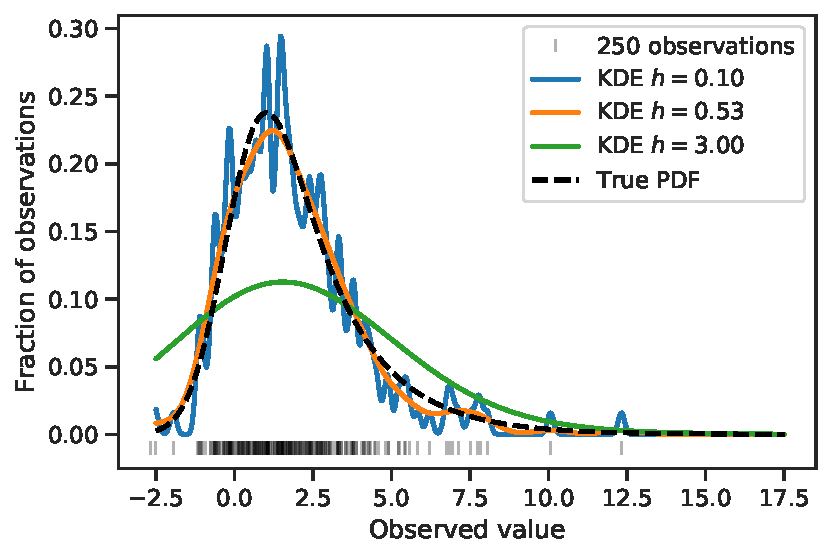
\includegraphics{figures/snemo_kde/1d_hist_example.pdf}
    \caption{Example of a kernel density estimate of a 1-dimensional, non-Gaussian distribution. The ticks represent the $n=250$ observations drawn from the true distribution shown with the black dashed line. The blue, orange, and green lines represent KDEs with increasing bandwidth sizes.}
    \label{fig:1d_hist}
\end{figure}

\subsubsection{Bandwidth Selection with Cross-validation}
There are some general rules-of-thumb for selecting an optimal bandwidth; for example, Silverman's rule of thumb:
$$h= 0.9\times\min\left(\hat{\sigma}, \frac{\textrm{IQR}}{1.34}\right) \times n^{-1/5}$$
where $\hat{\sigma}$ is the standard deviation of the sample, $\textrm{IQR}$ is the interquartile range of the sample, and $n$ is the number of data points in the sample \citep{Silverman1986}. This rule can perform quite well in most circumstances. However, these types of rules-of-thumb generalize quite poorly when the data is highly non-Gaussian (e.g. multi-modal distributions) or when the dimensionality of the data is high.

Another way to find the best bandwidth parameter is to try several values of the parameter and compare the results via some metric. A commonly used method for performing this type of evaluation is $k$-fold cross-validation. In $k$-fold cross-validation, we split the sample into $k$ groups. We then hold one of these groups out and train the model on the examples in the remaining $k-1$ groups. The model is then evaluated on the examples in the held-out set. This process is repeated until each example in the data set has been used in the training and validation. The overall model evaluation is then usually taken to be the mean of the evaluation metrics found in each of the cross-validation rounds, and the standard deviation of these metrics can be used to estimate the uncertainty on that metric.

A simple metric to use in the case of KDE is the sum of the log probabilities of the test data under the model. If the probability distribution resulting from the KDE is overfit (the bandwidth is too narrow), then the log probability of data points in the held-out set (which are drawn from the same underlying probability distribution) will be much lower than expected. The same would be true if the bandwidth was too wide and the model was underfitting the data, as long as the probabilities are normalized.

Using these techniques on our toy example from above, we find an optimal bandwidth of 0.53, as evidenced by the maximum at this point in Fig. \ref{fig:1d_bandwidth_opt}, plotting the total log probability of the $k$-folds as a function of bandwidth parameter.

\begin{figure}
    \centering
    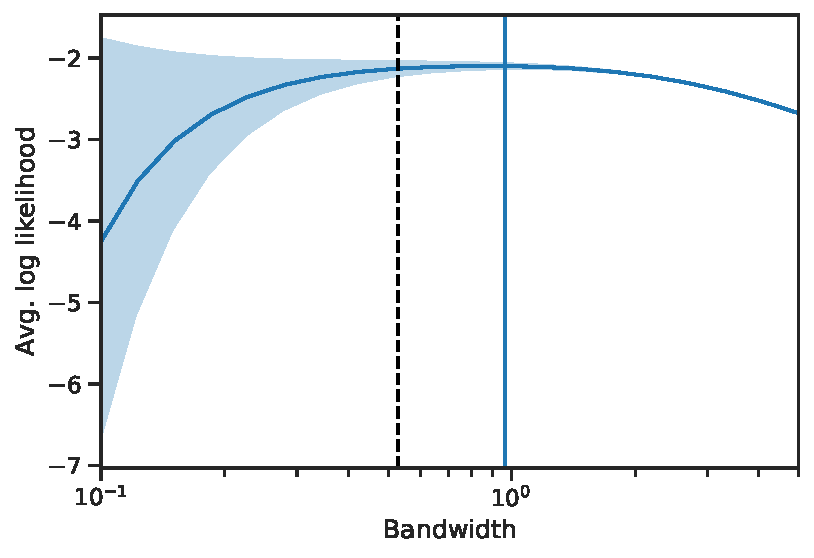
\includegraphics{figures/snemo_kde/1d_bandwidth_example.pdf}
    \caption{Results from 5-fold cross-validation for the example distribution and data shown in Fig. \ref{fig:1d_hist}. The blue line and shading show the mean and standard deviation of the normalized scores from all of the cross-validation subsets. The vertical blue line shows the location of the maximum score. The dashed black line shows the location of the Silverman's rule-of-thumb estimate for the optimal bandwidth.}
    \label{fig:1d_bandwidth_opt}
\end{figure}

\subsection[KDE in d Dimensions]{KDE in $d$ Dimensions}
The case in $d>1$ is quite similar to the 1-dimensional case. The kernel, though, is now in $d$ dimensions, and as such, the bandwidth is no longer a single parameter but a $d\times d$ symmetric matrix describing the bandwidth in each dimension along with the correlations between dimensions. The higher-dimensional case is further complicated by the so-called ``curse of dimensionality", where the sparseness of the data in the higher dimensional space causes the density estimate to converge more slowly. We will explore this first detail with a similar toy model to that used in \ref{sec:1d} but in 2 dimensions for ease of visualization.

\subsubsection{Transforming the Data for Bandwidth Estimation}
Consider a 2-dimensional sample drawn from a bivariate Gaussian distribution with mean $\bm{\mu}$ and covariance $\bm{\Sigma}$ (i.e. $(y_1, y_2)\sim\mathcal{N}(\bm{\mu}, \bm{\Sigma})$) and then consider a non-linear transformation to that sample, transforming $y_2$ to $z_2 = \exp(y_2)$. 

This example joint distribution is correlated and nonlinear, and as such works as a good test of the power and limitations of our methodology. We start by making estimates width a Gaussian kernel for a range of bandwidths as we did in the 1-dimensional case, giving us the results shown in Fig. \ref{fig:2d_scatter_unscaled}. However, the standard \verb|sklearn| implementation of the kernel density estimator incorrectly assumes that covariance matrix of the kernel is proportional to the identity matrix, so in our $k$-fold cross-validation, we are tuning a single bandwidth parameter $h$.

\begin{figure}
    \centering
    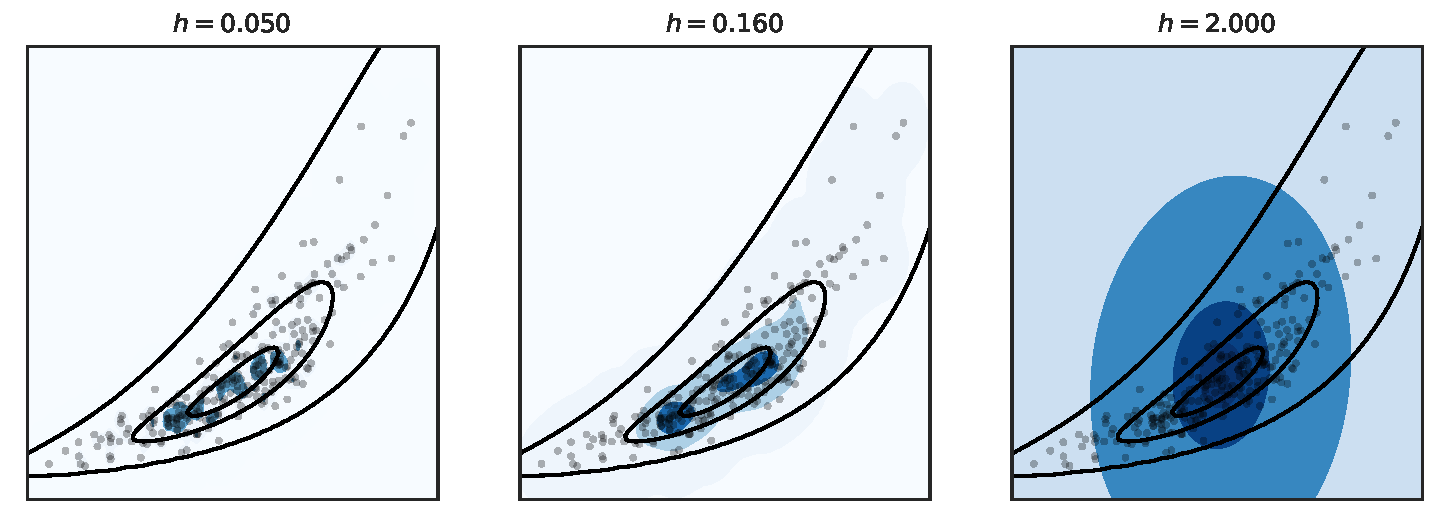
\includegraphics[width=0.9\textwidth]{figures/snemo_kde/2d_scatter_no_scaling.pdf}
    \caption{Example kernel density estimates in 2 dimensions for a joint probability distribution that is correlated and non-Gaussian. The $n=250$ data points are shown as black dots. The black contour lines show the true 1, 2, and 3 $\sigma$ contours, while the fading shades of blue show the 1, 2, and 3 $\sigma$ estimates of the KDE. In each of these examples, we assume a Gaussian kernel with no covariance terms.}
    \label{fig:2d_scatter_unscaled}
\end{figure}

We can see in the central panel of this figure that even the best-fit value of $h=0.143$ obtained from $k$-fold cross-validation is not a very good estimate of the true joint probability density. In particular, the density estimate makes the distribution appear multimodal. This occurs because the kernel does not reflect the full range of scales in the different dimensions of the space, so it takes on an $h$ value that reflects an average length scale.

We can improve our estimate by allowing the data to dictate the form of the kernel. We want to understand the relative fractions of the dispersion of the data in each dimension, as well as how the data covaries in each dimension. This will allow us to create a Gaussian kernel that is more reflective of the data, and therefore give us a better fit. We do this by finding a whitening transformation of the data, i.e. a transformation $W$ that turns our data matrix $X$ with covariance $\Sigma_X$ into a data matrix $Y=WX$ with covariance $\Sigma_Y=\mathbb{I}$. With this whitening transformation, we can reproject our data into whitened space, fit the KDE as usual, and then apply the inverse transformation to the KDE sample to obtain a KDE with a tuned kernel that matches the data.

A commonly used whitening matrix is $W = \Lambda^{-1/2}U^\top$, where $\Lambda$ is the diagonal matrix of eigenvalues and $U$ is the matrix whose columns are the eigenvectors of the covariance matrix $\Sigma_x$ (see proof in Appendix \ref{app:whitening_matrix_proof}). Using this transformation, we can complete the process of transforming our data, fitting the KDE, and inverting the transformation to find a better fit to the data distribution. Fig. \ref{fig:2d_rescaling_process} shows an explicit example, and Fig. \ref{fig:2d_scatter_scaled} directly compares the estimates of joint probability distribution that come from fits with and without this process. The predicted likelihood distribution is no longer multimodal, and the overall similarity between the distributions is improved.

\begin{figure}
    \centering
    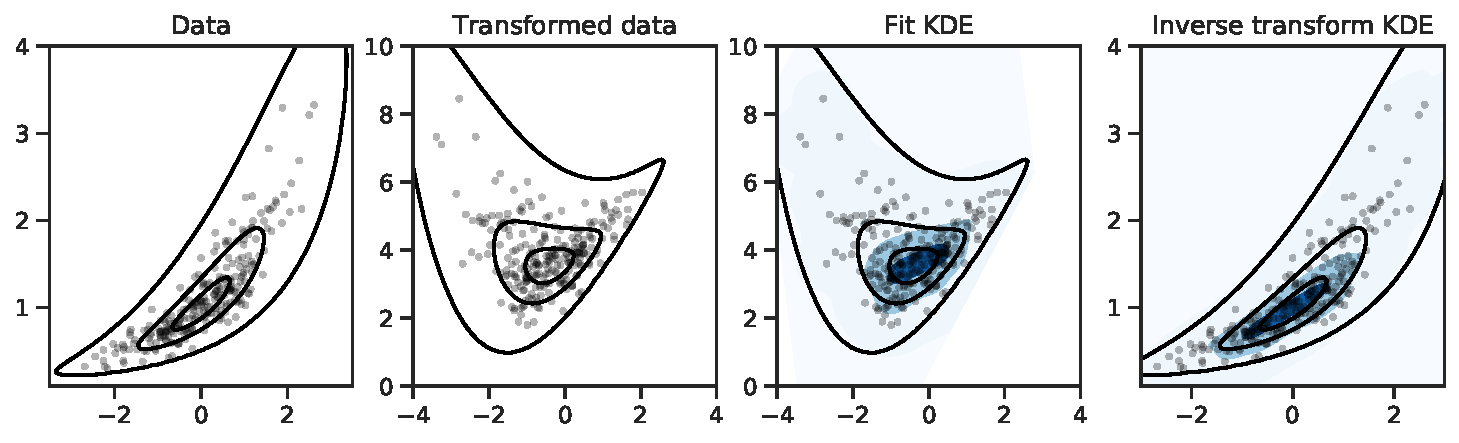
\includegraphics[width=0.9\textwidth]{figures/snemo_kde/2d_rescaling_process.pdf}
    \caption{The process of transforming the data to use a kernel that captures the data covariance. The first panel shows the data in the original coordinates. The second panel shows the data after being transformed by the whitening transformation. The third panel shows the KDE fit with a normal Gaussian kernel, and the final panel shows the data and the KDE reprojected back into the original coordinates. In each panel, the same data points are shown as black dots. The true 1, 2, and 3 $\sigma$ contours are shown in differing shades of blue. The black lines indicate the 1, 2, and 3 $\sigma$ confidence intervals of the best-fit KDE.}
    \label{fig:2d_rescaling_process}
\end{figure}

\begin{figure}
    \centering
    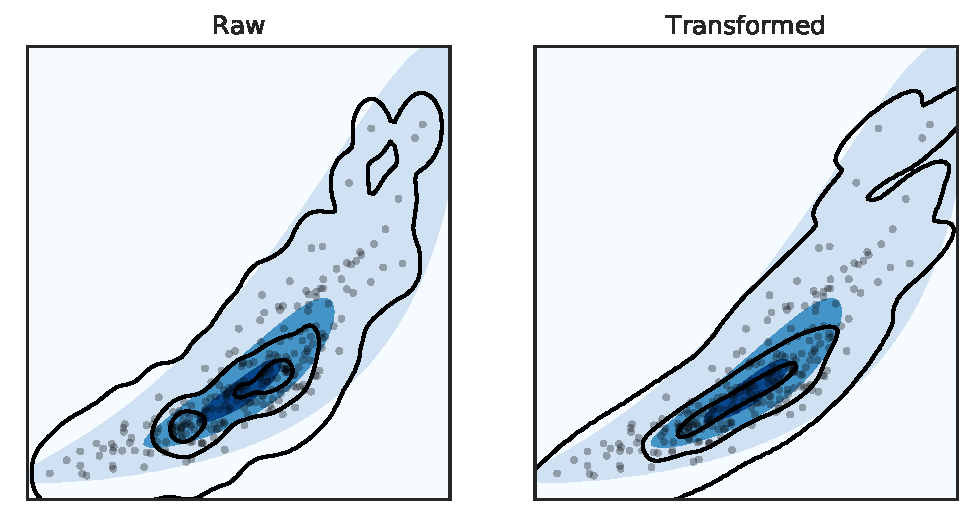
\includegraphics[width=0.9\textwidth]{figures/snemo_kde/2d_scatter.pdf}
    \caption{Comparison of the final KDE for our toy example using a) the best-fit Gaussian kernel with no covariance transformation and b) the best-fit Gaussian kernel with whitening applied. In both panels, the blue shading indicates the 1, 2, and 3 $\sigma$ contours of the true toy model distribution, and the black lines indicate similar contours for the kernel density estimates of the distribution.}
    \label{fig:2d_scatter_scaled}
\end{figure}

\section{Modeling the Data and Making Mock Observations}
\label{sec:making_mocks}
\subsection{Comparing Parameter Distributions}
We apply the multidimensional KDE fitting process laid out in the previous section to the spectral model parameter measurements found in Section \ref{sec:data}. Corner plots of the data points and similarly sized samples drawn from the resulting transformed KDE are shown in Figs. \ref{fig:salt2_sample}-\ref{fig:snemo15_sample}.

\begin{figure}
    \centering
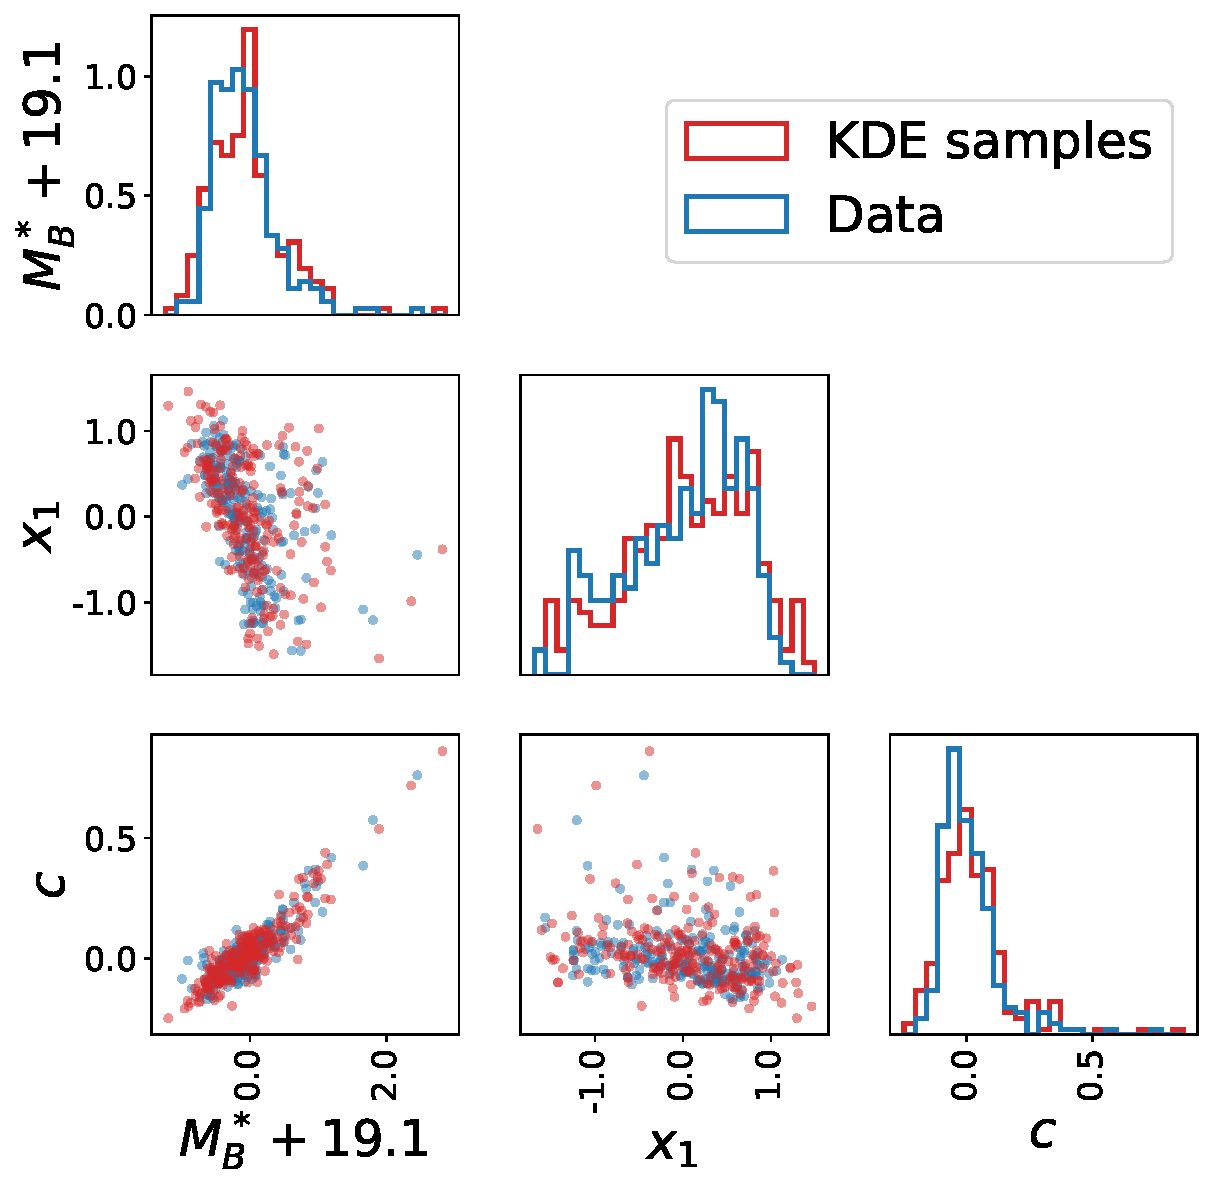
\includegraphics[width=0.9\textwidth]{figures/snemo_kde/salt2_corner.pdf}
    \caption{Corner plot showing the joint and marginal parameter distributions of the SALT2 parameters for the SNfactory data set (in blue), as well as the distribution of samples drawn from the KDE trained on these data (in red).}
    \label{fig:salt2_sample}
\end{figure}

\begin{figure}
    \centering
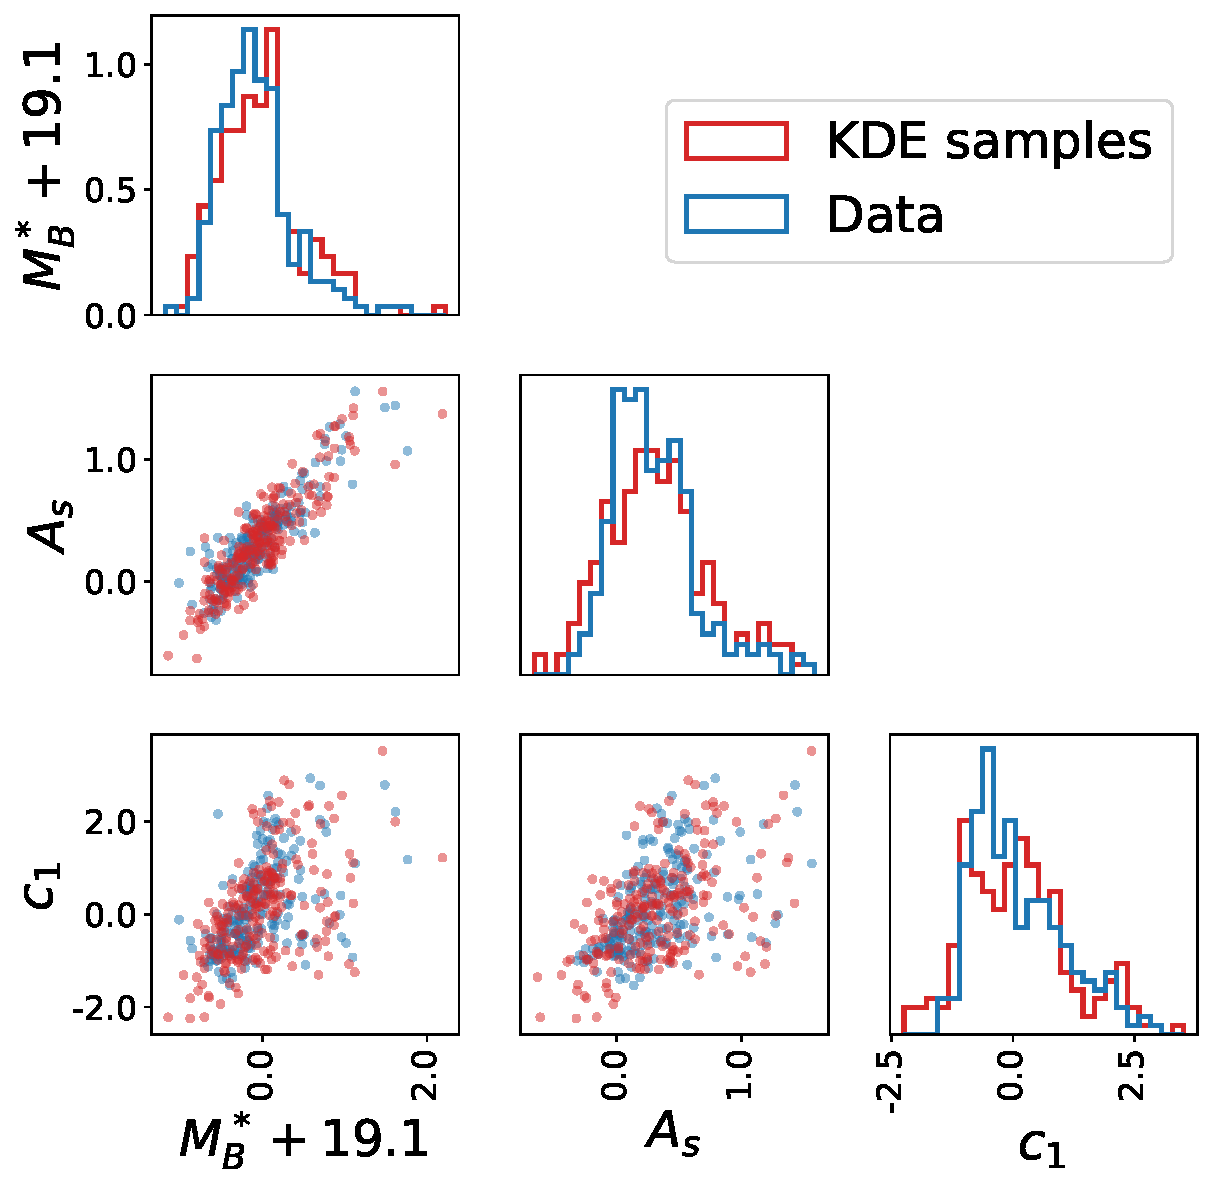
\includegraphics[width=0.9\textwidth]{figures/snemo_kde/snemo2_corner.pdf}
    \caption{Same as Fig. \ref{fig:salt2_sample}, but for SNEMO2}
    \label{fig:snemo2_sample}
\end{figure}

\begin{figure}
    \centering
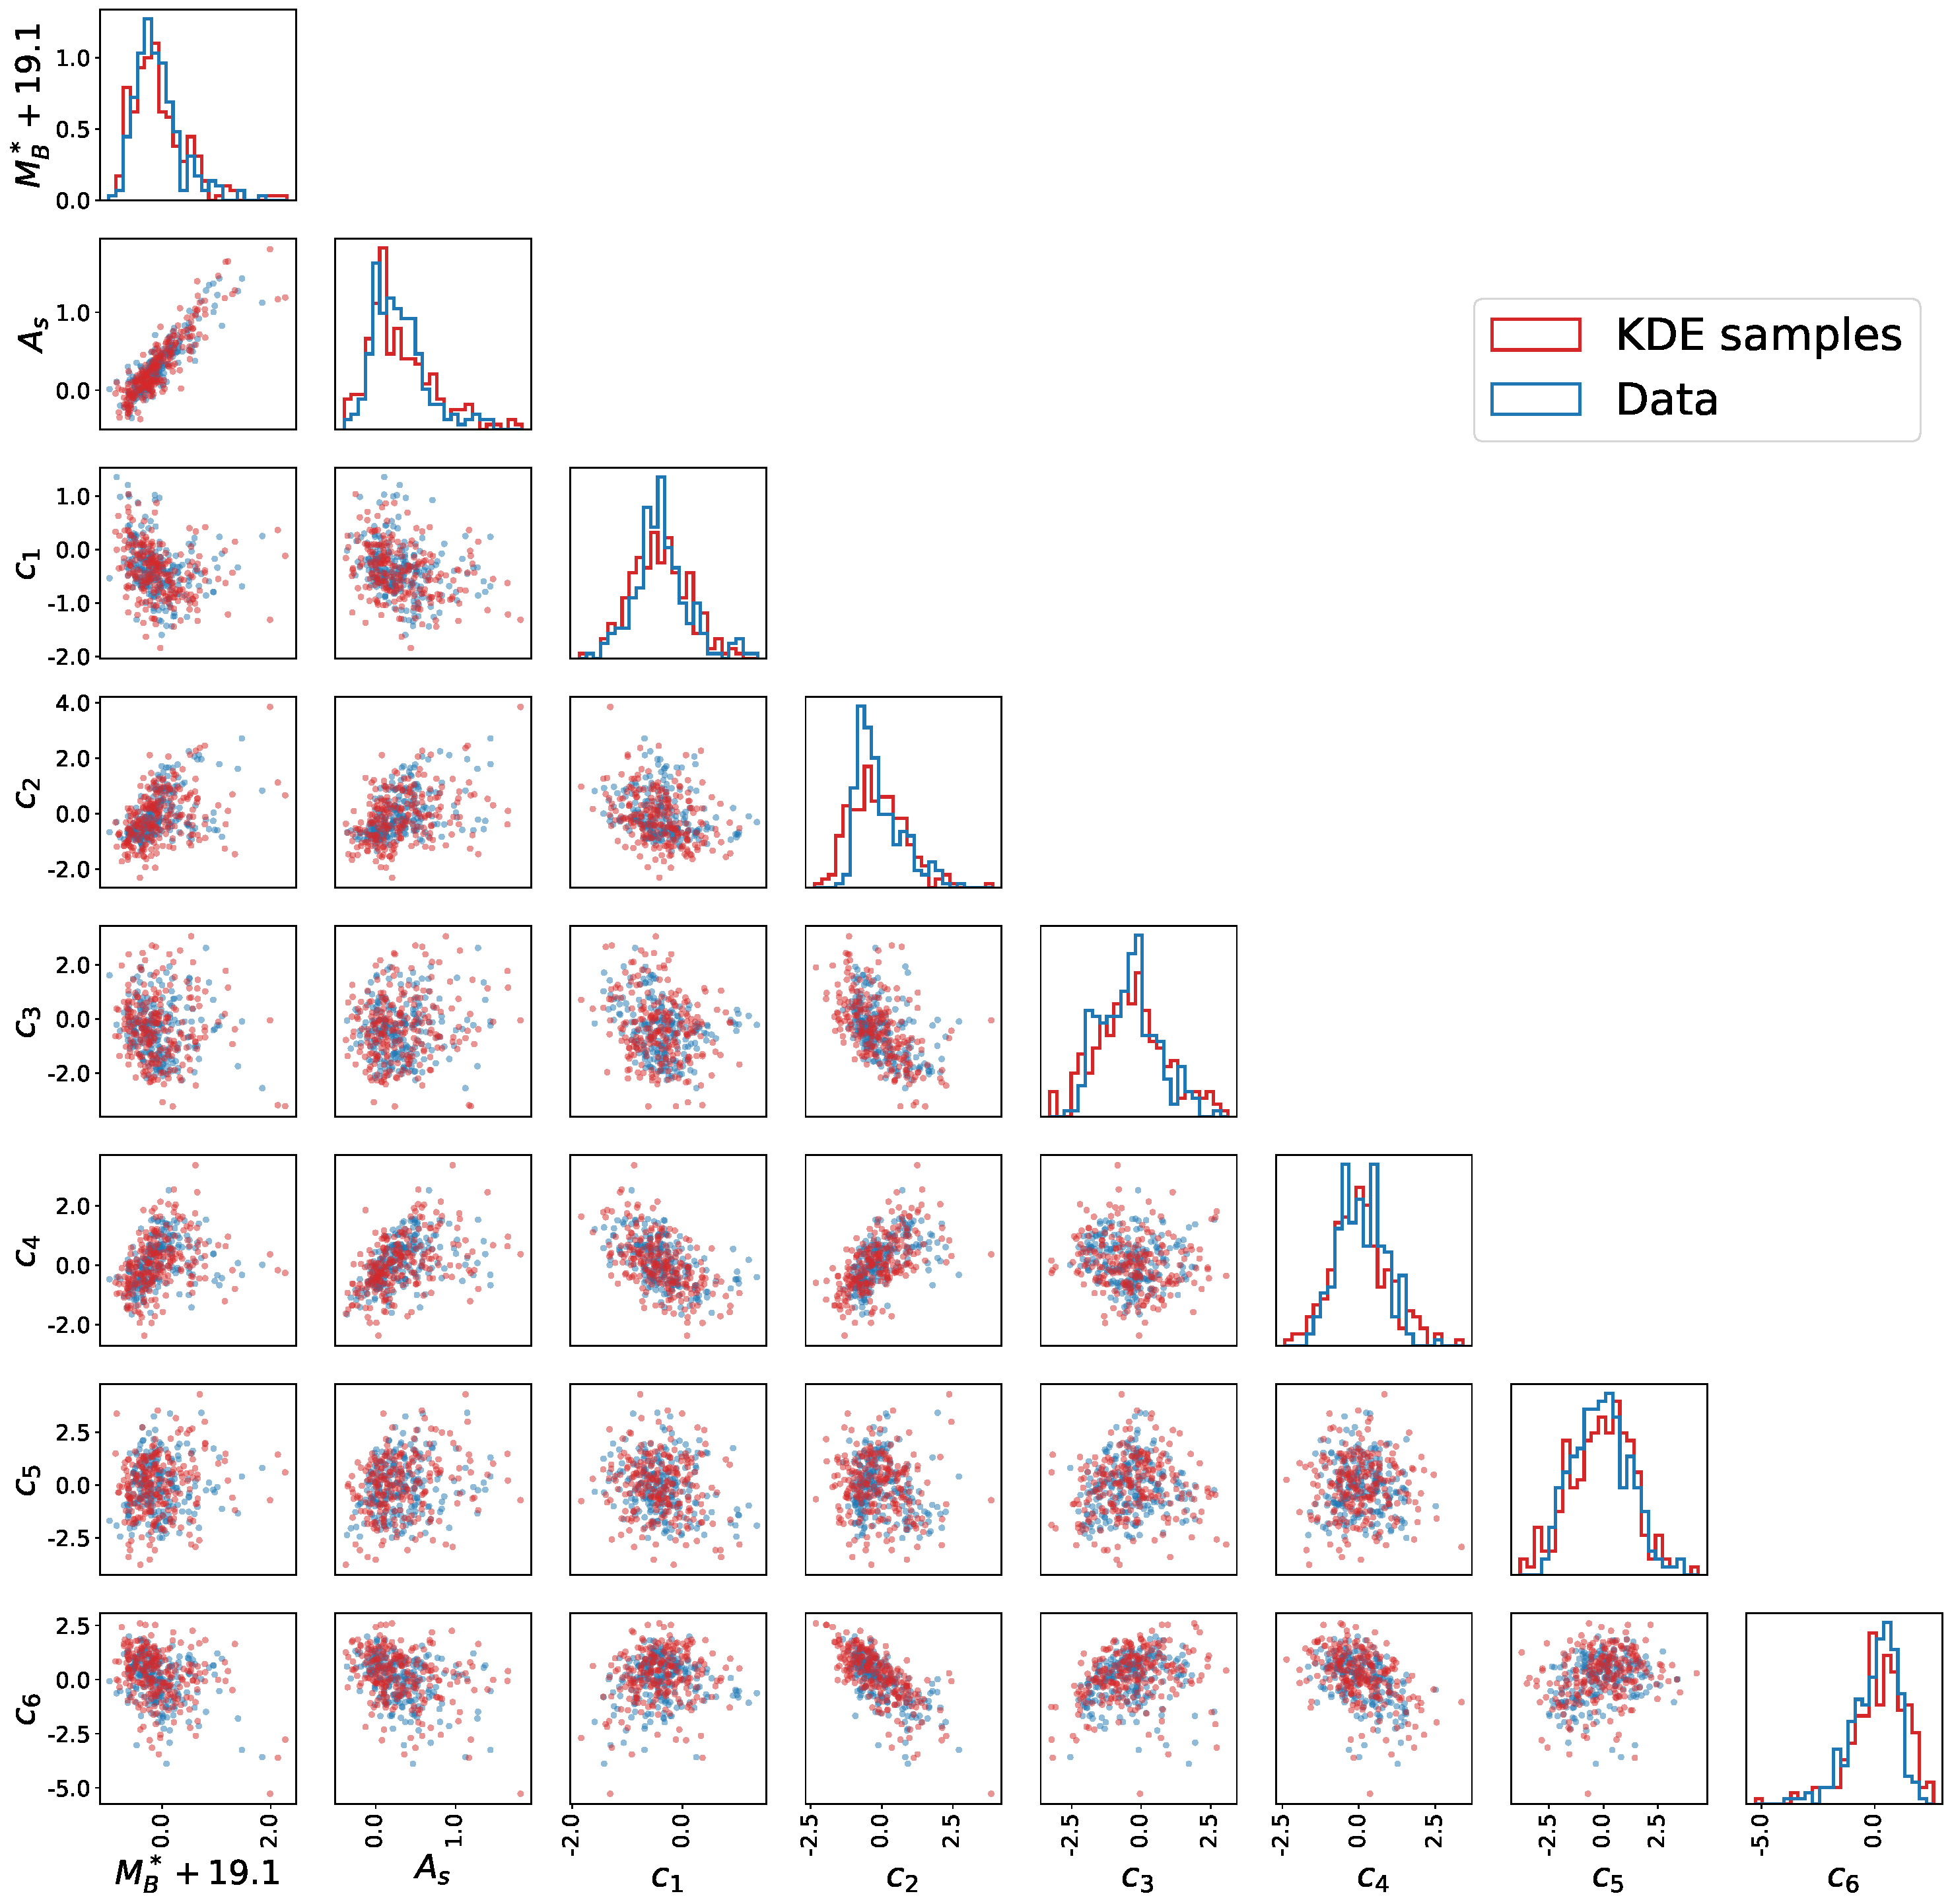
\includegraphics[width=0.9\textwidth]{figures/snemo_kde/snemo7_corner.pdf}
    \caption{Same as Fig. \ref{fig:salt2_sample}, but for SNEMO7}
    \label{fig:snemo7_sample}
\end{figure}

\begin{figure}
    \centering
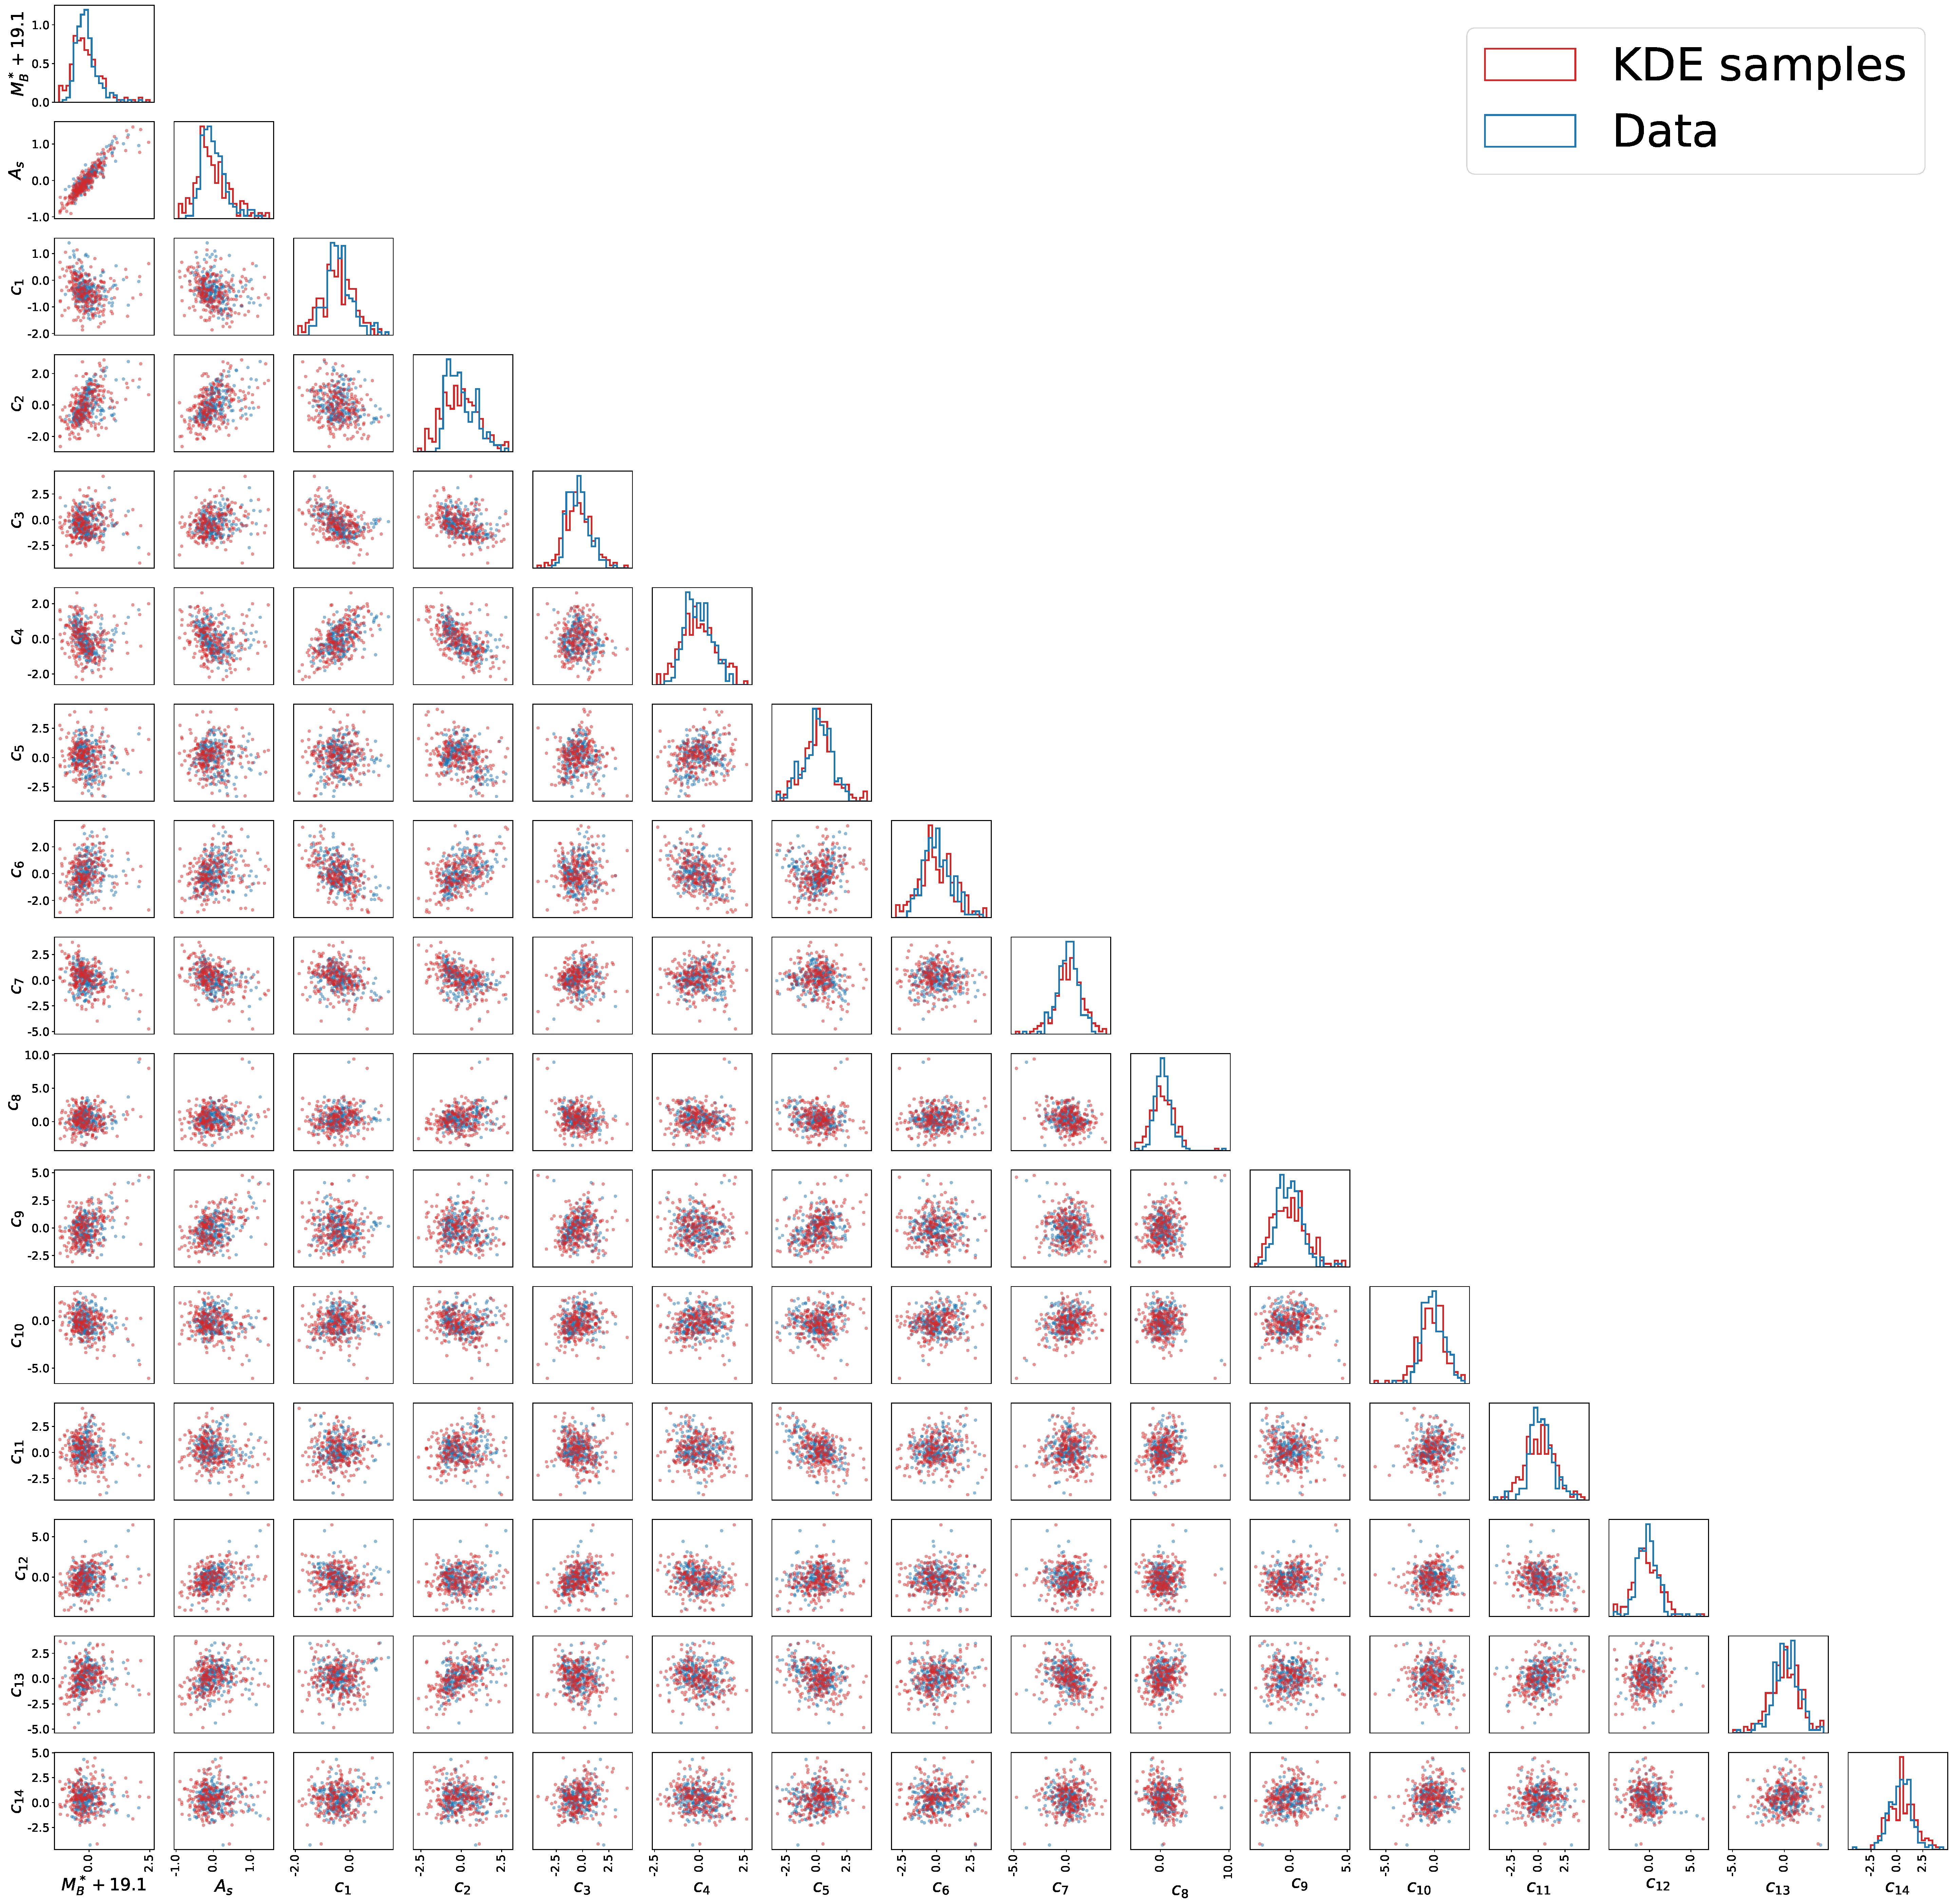
\includegraphics[width=0.9\textwidth]{figures/snemo_kde/snemo15_corner.pdf}
    \caption{Same as Fig. \ref{fig:salt2_sample}, but for SNEMO15}
    \label{fig:snemo15_sample}
\end{figure}

In order to quantify the advantage of using this kernel density estimate over a simpler model, like a multivariate Gaussian for example, we use the two-sample Cram\'{e}r distance \citep{Cramer1928} to measure the difference between the cumulative distribution function of the data and the estimated distributions from empirical cumulative distribution functions of the samples.
The Cram\'{e}r distance $\omega$ between a probability distribution with the empirical cumulative distribution function $F(x)$ and a second probability distribution with the empirical cumulative distribution function $G(x)$ is defined by
\begin{equation}
    \omega^2 = \displaystyle \int_\infty^\infty [F(x)-G(x)]^2 dx
\end{equation}
Smaller values indicate closer agreement between the two distributions.

This distance metric has the advantage over other more well-known test statistics (like the Kolmogorov-Smirnov statistic) of being sensitive to differences in the shape of distributions beyond just shifts in the mean or standard deviation, particularly in the tails of the distribution. This is ideal for our task because we want our parameter space estimates to match the true distribution across all portions of parameter space.

Calculating this distance in many dimensions is possible, but computationally difficult because of memory limitations in calculating large dimensional histograms. Therefore, we chose to compare each of the \emph{marginalized} distributions of each spectral model parameter. The Cram\'{e}r distances between the spectral model parameter marginal distributions from the best-fit KDE and from the data, as well as corresponding distances where a simple multivariate Gaussian replaces the KDE, are presented in Fig. \ref{fig:distances}.

\begin{figure}
    \centering
    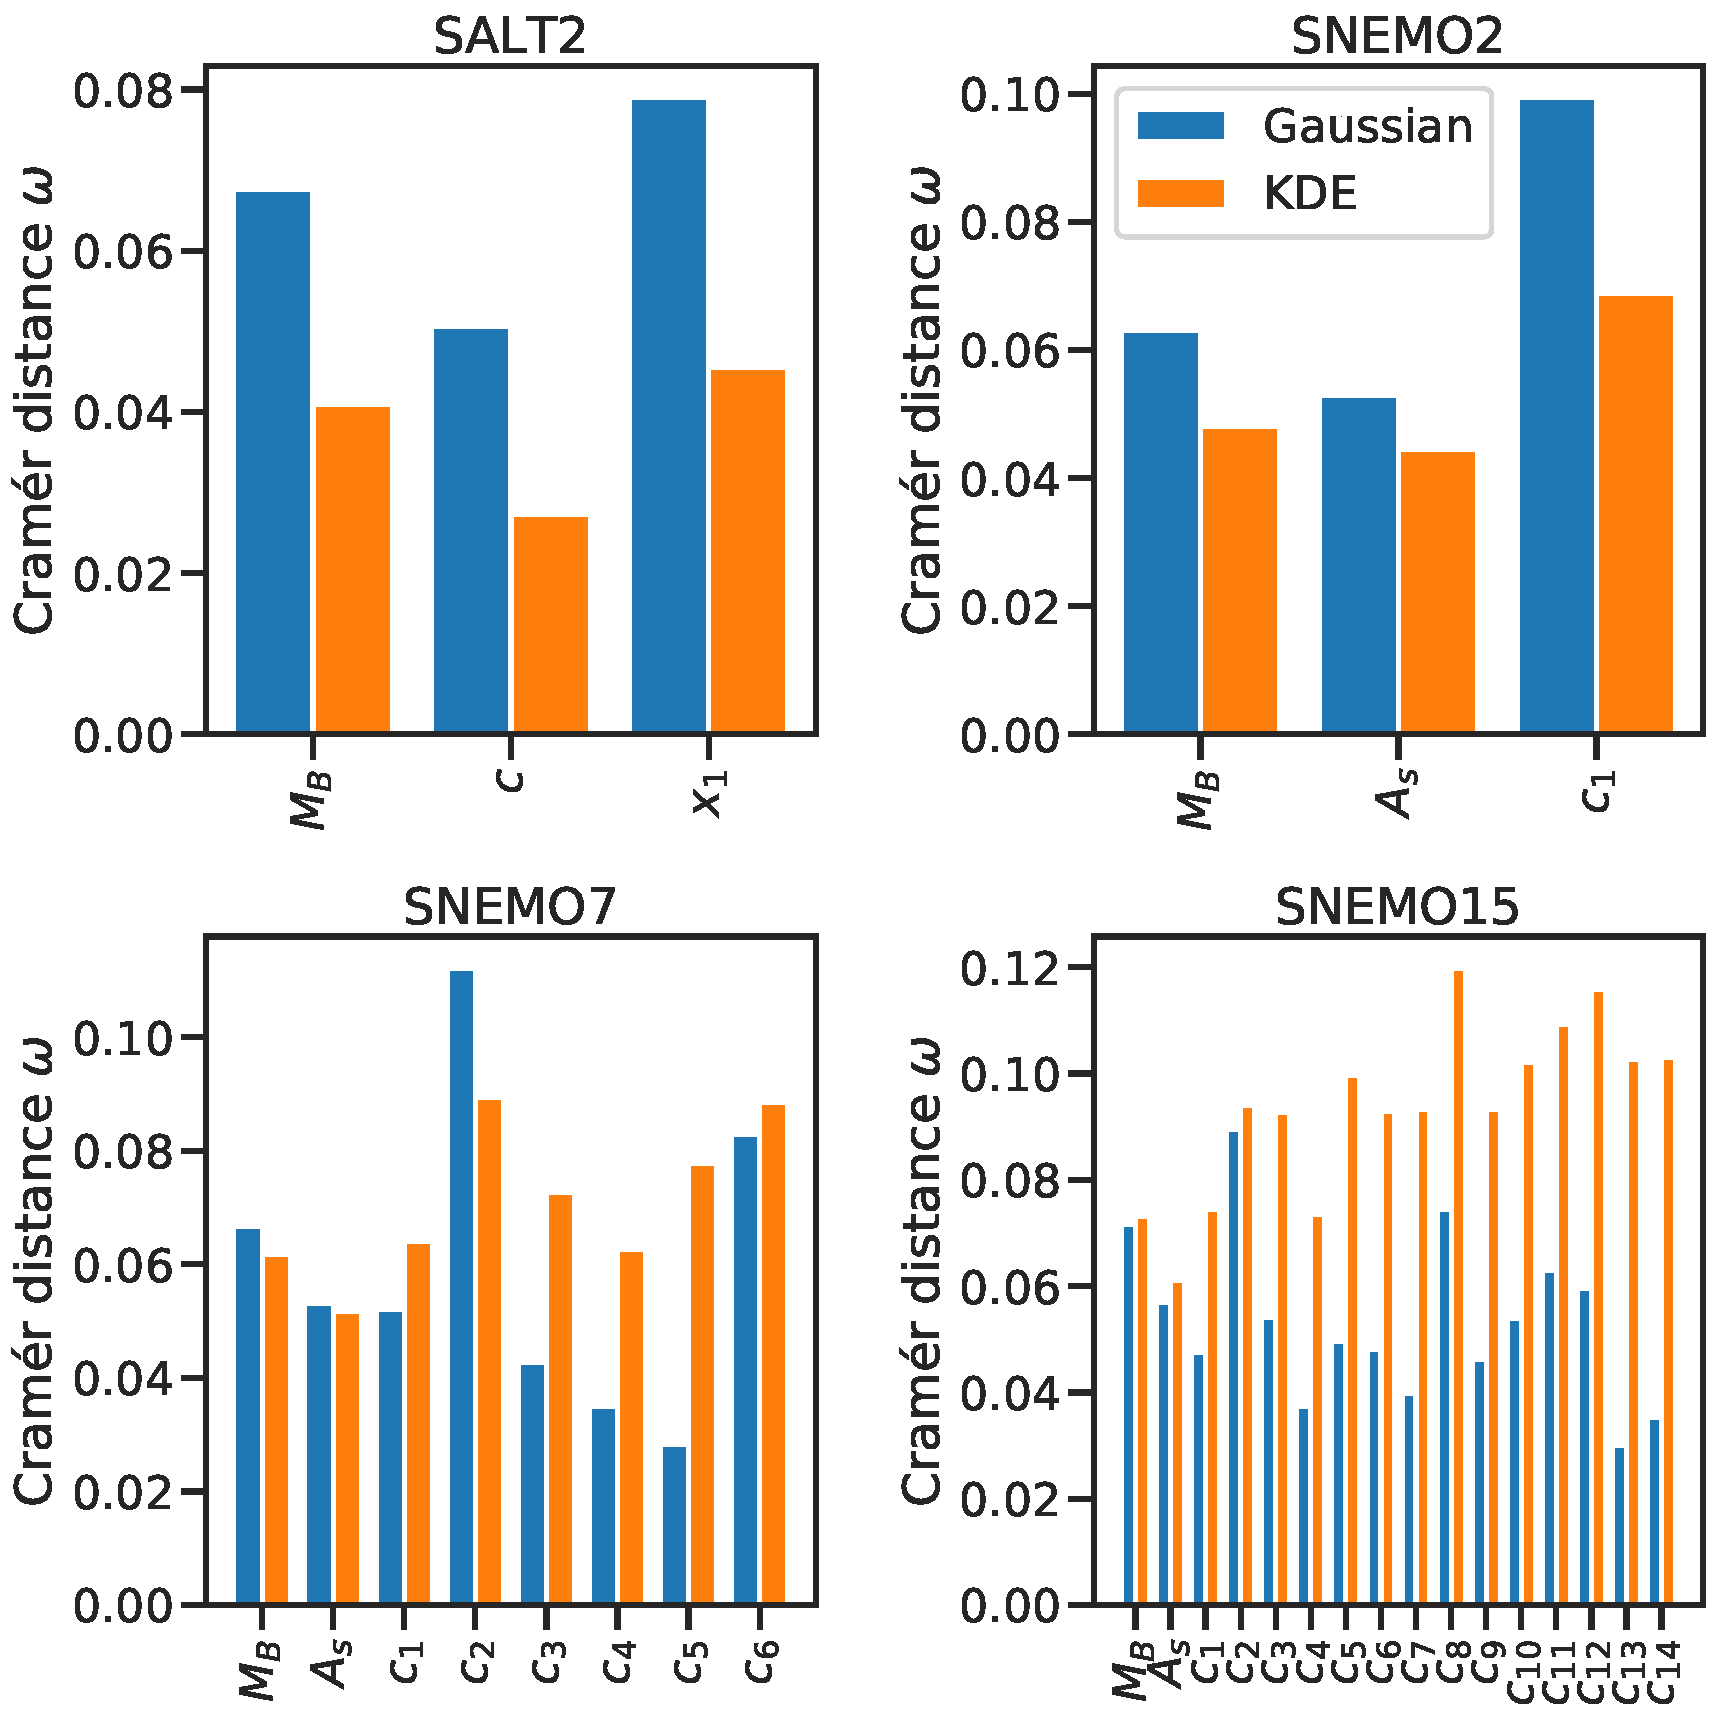
\includegraphics[width=0.9\textwidth]{figures/snemo_kde/cramer_distances_param_space.pdf}
    \caption{Cram\'{e}r distances between the empirical marginal distributions functions of the data sample and samples from a multivariate Gaussian (blue) and samples from the KDE (orange) for each parameter in each of the spectral models studied.}
    \label{fig:distances}
\end{figure}

In the lower-dimensional models (SNEMO2 and SALT2), the marginal distributions of the parameters found with the KDEs match those from the data much better than those drawn from a simple multivariate Gaussian. For SNEMO7, some of the marginalized parameter distributions, like $c_2$, are better described by the KDE than the Gaussian. Others, however, are better approximated by a Gaussian distribution. For SNEMO15, each of the marginalized parameter distributions are better modeled by Gaussians than they are by the marginalized KDEs. 

It is important to note that the metric we are using uses only the information from the marginalized probability. distributions, and therefore cannot account for skewness and non-Gaussianity in the joint probability distributions. As an example of this effect, we show the observed 2-dimensional joint distribution of SNEMO15 $A_s$ and $c_1$, along with contour plots of the same distribution given by the KDE and a multivariate Gaussian in Fig. \ref{fig:snemo15_joint_example}. While the Cram\'{e}r distance between the data and the marginalized KDE distributions of these two parameters is larger than the distance between the data and the marginalized Gaussian distribution, we see visually that the KDE seems to better capture the deviations from pure Gaussianity in the joint distributions, as evidenced by the closer agreement of the modes of the distributions and incorporation of larger tails in the distribution. Moreover, we will see in Section \ref{sec:spec_diversity} that using the KDE to model the spectral model parameter space allows us to capture a more realistic range of spectral feature measurements. The distances presented are meant to serve as a rough heuristic for the agreement between the distributions found by this technique and the data. A more detailed look, perhaps exploring the Cram\'{e}r distances in the two-dimensional distributions, is left to future work.

\begin{figure}
    \centering
    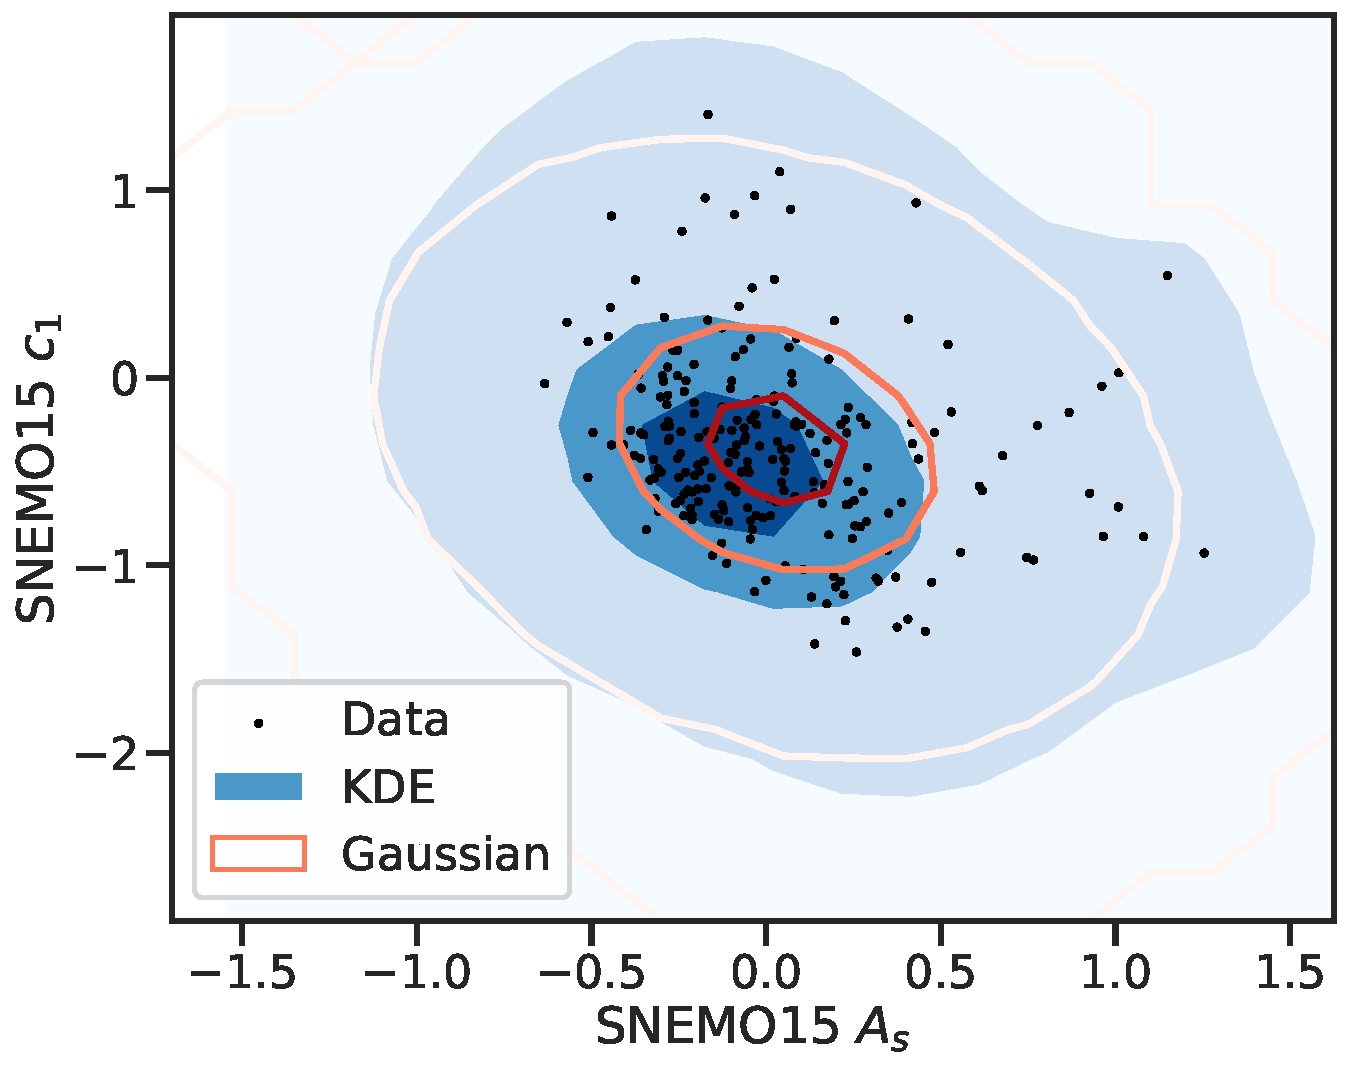
\includegraphics[width=0.9\textwidth]{figures/snemo_kde/snemo15_nongaussian_example.pdf}
    \caption{Comparison of the KDE estimate (blue filled contours representing the 68th, 95th, and 99th percentiles of samples drawn from the full 16-dimensional estimate) and multivariate Gaussian estimate (similarly spaced red line contours) of the joint probability distribution between SNEMO15 $A_s$ and $c_1$. While the Gaussian estimate shows a closer agreement in the marginal distribution of these parameters, according to the Cram\'{e}r distance (see Fig. \ref{fig:distances}), the KDE seems to allow a wider variety of values and better captures the skewness of this data because it is not constrained to match the Gaussian form.}
    \label{fig:snemo15_joint_example}
\end{figure}

\subsection{Generating Mock Observations}
With the modeled latent space in hand, we can easily obtain new SN Ia instances to use in further analyses by drawing from the underlying joint probability distribution, calculating the scaling coefficient $x_0$ or $c_0$, and plugging the resulting parameters into Eqn. \ref{eqn:salt_flux_model} or \ref{eqn:snemo_flux_model}. This process gives us a grid of flux values across the model wavelength range (3305-8685 \AA for the SNEMO models or 2000-9200 \AA for SALT2) and phase range (-10 to +40 rest-frame days after maximum brightness for the SNEMO models or -20 to +50 rest-frame days for SALT2).

As explained in Section \ref{sec:data}, we have modeled the absolute magnitude, rather than the redshift-dependent scaling parameters $x_0$ and $c_0$. To convert the $M_B^* + 19.1$ value to $x_0$ or $c_0$, we first choose a redshift $z$ for the supernova instance based on the needs of our analysis and calculate $m_B$, the peak apparent magnitude of an object at that redshift with $c_0=1$ and all of the remaining parameters set to values determined by the draw from the modeled distribution. We also calculate the desired apparent magnitude, $m_B^*$, by adding the distance modulus $\mu(z)$ from our fiducial cosmology to the apparent magnitude $M_B^*$ drawn from the modeled distribution. The final scale factor is then given by 
$$c_0 = 10^{-0.4(m_B^*-m_B)}.$$

Once we have our grid of flux values $f(\lambda, p)$, we can then easily synthesize spectroscopy or photometry of any resolution or signal-to-noise ratio using a tool like \verb|sncosmo|\footnote{\url{https://sncosmo.readthedocs.io/en/v2.1.x/}}. In Fig. \ref{fig:example_prism_spec}, we show spectra of an example object at redshift $z=0.775$ with intrinsic flux determined by a draw from the KDE model of the SNEMO15 model parameters, using the spectral resolution of the proposed Roman Space Telescope prism spectrograph and signal-to-noise equivalent to an exposure time of roughly one hour. Fig. \ref{fig:example_roman_lc} shows the same object but observed through photometry in the bandpasses proposed for the Roman Wide Field Instrument for a similar exposure time. 

\begin{figure}
    \centering
    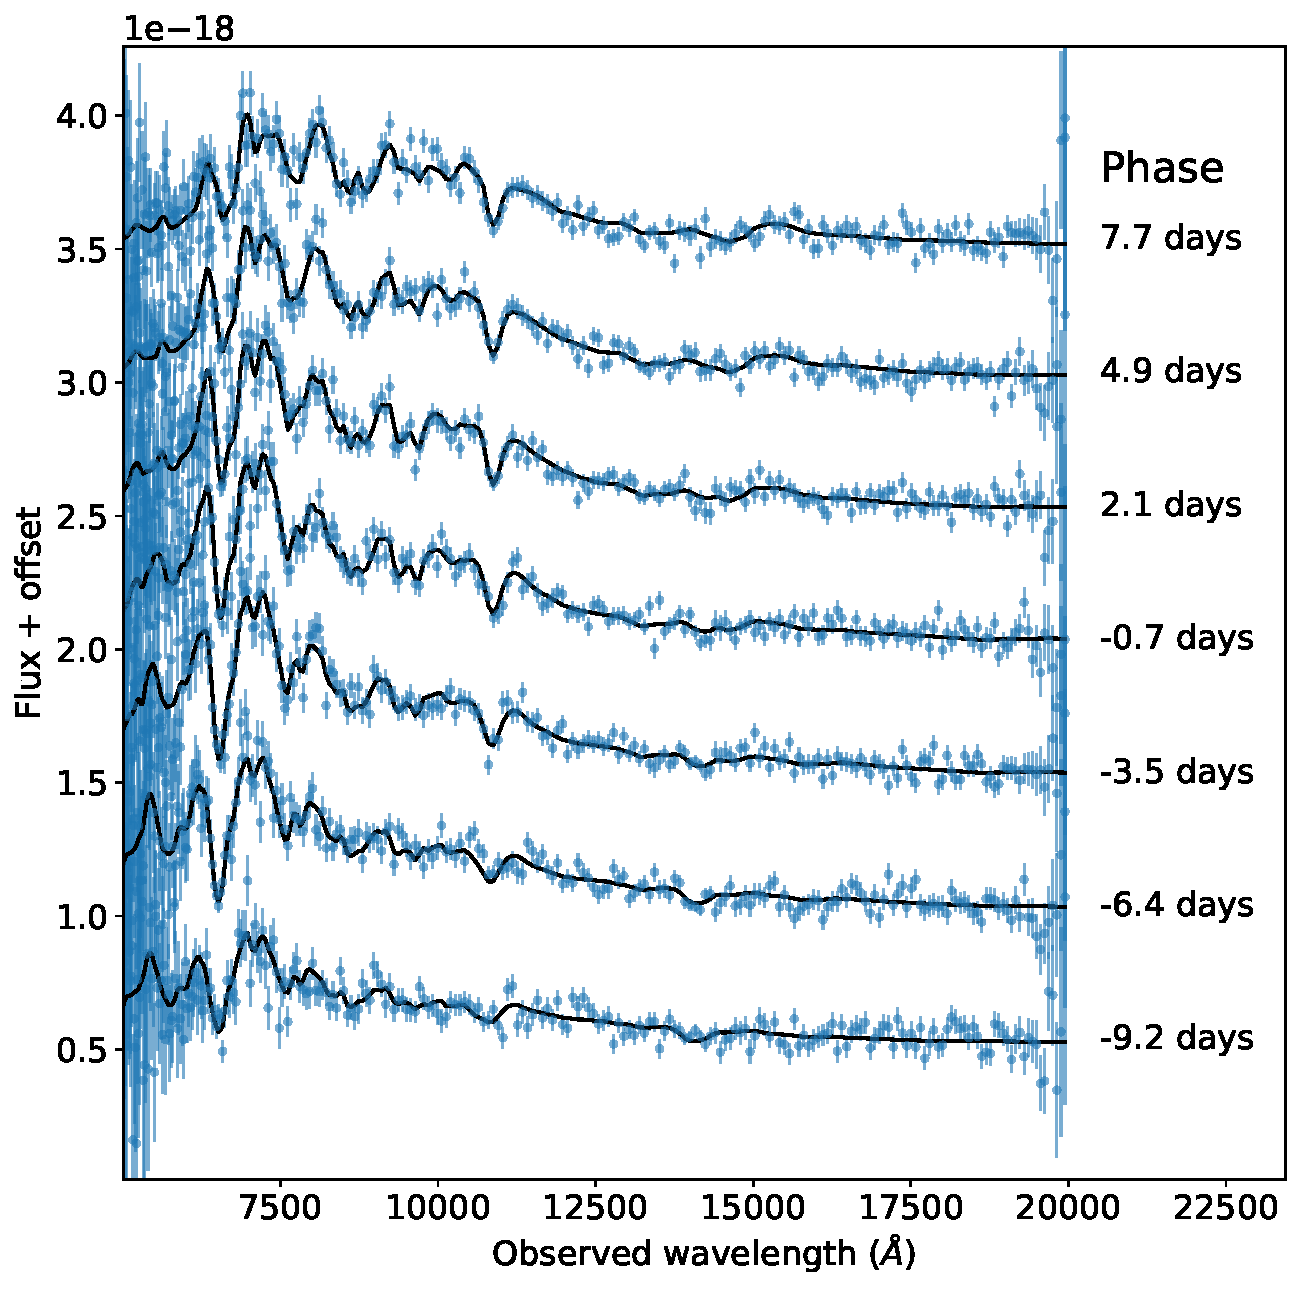
\includegraphics[width=0.9\textwidth]{figures/snemo_kde/example_roman_spec.pdf}
    \caption{A series of synthesized spectral observations at a range of phases for a single object at redshift $z=0.775$ generated from a random draw from the SNEMO15 KDE. The resolution matches the proposed design of the Roman Space Telescope prism spectrograph, and the signal-to-noise ratio representing the level that could be obtained with an hour of exposure time.}
    \label{fig:example_prism_spec}
\end{figure}

\begin{figure}
    \centering
    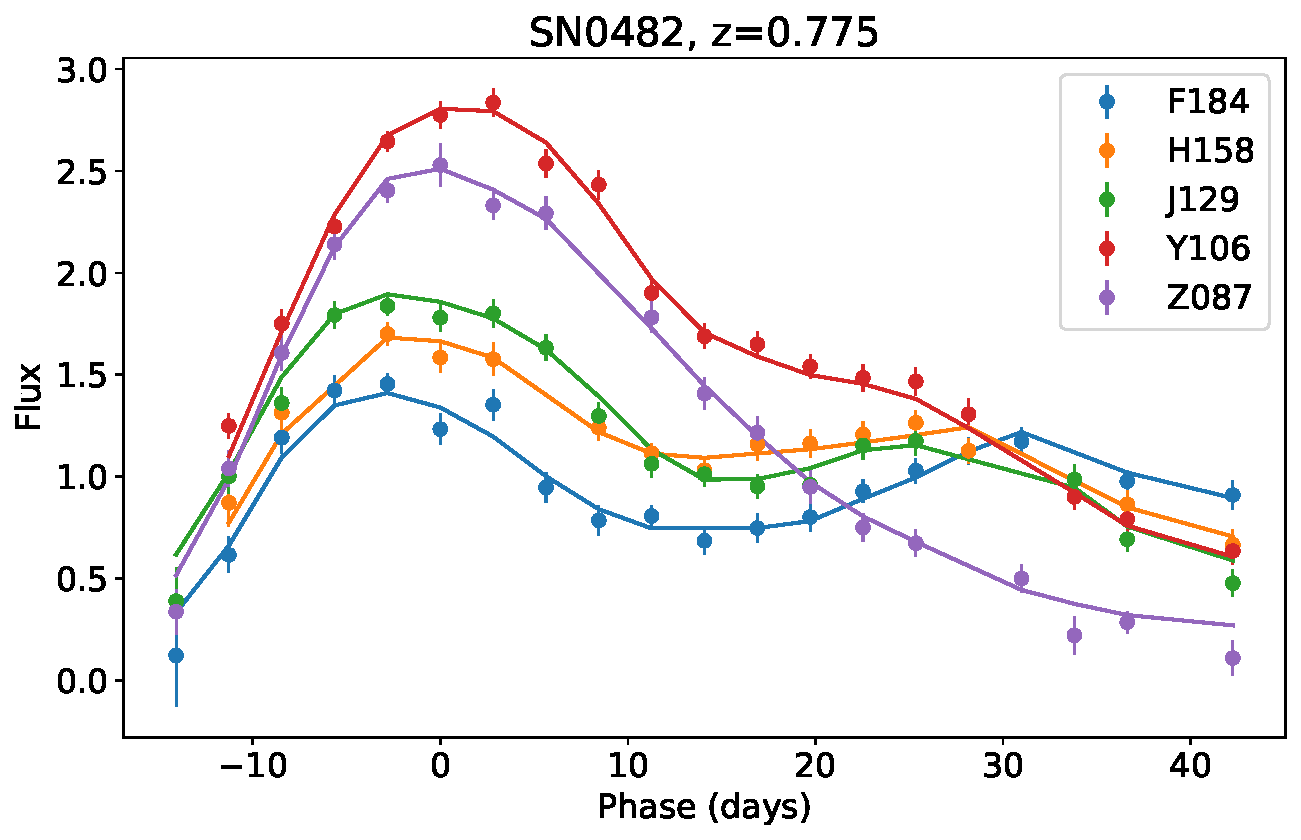
\includegraphics[width=0.9\textwidth]{figures/snemo_kde/example_roman_lc.pdf}
    \caption{Synthetic photometry of the same object shown in Fig. \ref{fig:example_prism_spec}, but observed photometrically in the Roman Wide Field Instrument bandpasses.}
    \label{fig:example_roman_lc}
\end{figure}

\section{Evaluating Spectral Diversity}
\label{sec:spec_diversity}
As another means of quantifying the usefulness of this tool, as well as a concrete example of the kind of analysis that is uniquely enabled by both a non-parametric model of spectral model parameters and the use of higher-dimensional spectral models (SNEMO7 and SNEMO15), we compare the distributions of several spectral features measured from the training spectra to the those obtained with data simulated by the techniques introduced in this work. The development of the SNEMO models was largely motivated by the recognition that spectral models like SALT2 do not capture the full range of spectral variation that is seen in Type Ia supernovae \citep{Saunders2018}. This study aims to quantify how well higher-dimensional linear models and non-parametric models of the latent parameter space of these linear models can capture the non-linear features that may provide a better understanding of supernova standardization and supernova physics.

We chose to focus on the velocities and pseudo-equivalent widths of the CaIIH\&K doublet, the SiII5972 line, and the SiII6355 line at maximum brightness. These spectral indicators are commonly used in studies aiming to improve the standardization of supernova brightnesses beyond light curve shape and color, or to quantitatively subclassify Type Ia supernovae in order to gain a better understanding of their physics. The ejecta velocities of SNe Ia, measured by the line velocities of SiII6355 and CaIIH\&K, have been shown to correlate with their intrinsic colors \citep{FoleyKasen2011, FSK2011, Foley2012, Mandel2014}. The width of the SiII6355 line shows a similar correlation \citep{FSK2011}. Evidence of a correlation between the velocity of the SiII6355 line and Hubble residuals has been shown directly in \cite{Siebert2020}. All of these relationships can lead to potential redshift-dependent distance bias if left uncorrected. An example subclassification scheme using these parameters is the Branch classification scheme \citep{Branch2006}, which arranges SNe Ia by the widths of their SiII5972 and SiII6355 lines, showing that there is a wide range in spectral feature behavior within the Ia class. 

To measure these features from real data (with associated flux noise), we first smooth the spectrum by convolving the observed flux $f(\lambda)$ with a Gaussian window weighted by the inverse of the flux variance, as is done in \cite{Blondin2006}, to get a smoothed spectrum $f_s(\lambda)$. Simulated spectra have no noise, so we do not smooth them. We do however interpolate both the smoothed, observed data and the simulated spectra onto a wavelength grid with 0.1 \AA resolution. For each feature region, we define a pseudo-continuum by identifying the local maxima $\lambda_{b}$ and $\lambda_{r}$ in the wavelength ranges blueward and redward of each feature described in Table \ref{tab:spec_feat_info} and calculating the line that connects these two points. We divide the flux by that line to obtain the pseudo-continuum-removed local feature spectrum $f_c(\lambda)$. The velocity of each line is determined by finding the wavelength of the minimum of the pseudo-continuum-removed local feature spectrum ($\lambda_\text{min}$) and using this value in the relativistic Doppler formula along with the rest-frame minimum wavelength $\lambda_0$ listed for each feature in Table \ref{tab:spec_feat_info}:
\begin{equation}
    \frac{v}{c} = \frac{\left(\lambda_\text{min}/\lambda_0\right)^2-1}{\left(\lambda_\text{min}/\lambda_0\right)^2+1}
    \label{eqn:rel_doppler}
\end{equation}
The pseudo-equivalent width is calculated by integrating
\begin{equation}
    \text{pEW} = \displaystyle\int_{\lambda_b}^{\lambda_r} \left[1-\frac{f_s(\lambda)}{f_c(\lambda)}\right] d\lambda
    \label{eqn:pew}
\end{equation}.

\begin{table}[ht!]
    \centering
    \begin{tabular}{|c|c|c|c|}\hline
    Feature name & $\lambda_b$ range (\AA) & $\lambda_r$ range (\AA) & $\lambda_0$ (\AA)\\\hline
    CaIIH\&K & 3504 - 3687 & 3887 - 3990 & 3945\\
    SiII5972 & 5550 - 5681 & 5850 - 6015 & 5972\\
    SiII6355 & 5850 - 6015 & 6250 - 6365 & 6355\\\hline
    \end{tabular}
    \caption{Extrema limits and rest-frame minimum wavelengths for the spectral indicators studied.}
    \label{tab:spec_feat_info}
\end{table}
These indicators were measured from the spectrum of each supernova in our data set that was closest to the SALT2-predicted time of B-band maximum brightness, $t_0$. To minimize the impact of phase evolution of the features, we remove from the analysis all objects that do not have a spectrum within $\pm 5$ rest-frame days of $t_0$. This leaves 213 supernovae. Code to perform these measurements is publicly available through the \verb|spectral_lines| package\footnote{\url{https://github.com/sam-dixon/spectral_lines}}.

\subsection{Comparing Features Measured from Data and from Best-fit Spectral Models}
We would like to separate our quantification of how well the spectral flux models themselves are able to capture the full distributions of spectral features from how closely samples generated from the KDE models of the spectral model parameters mimic the true distribution. To answer the first question, we make measurements of the spectral features from noiseless, at-max spectra synthesized directly from the best-fit spectral model parameters for each supernova and each spectral model (presented earlier in Table \ref{tab:snemo_coefs}). We will refer to these measurements as the model measurements.

Fig. \ref{fig:model_vSi_recovery} shows histograms of the residuals between these model-measured velocity of SiII6355 ($v_{SiII6355}$ and the data-measured velocity for each object in our data set. We can see that as the number of model components increases, the scatter on these residuals decreases, indicating that the increased flexibility of these higher-dimensional spectral models allows them to capture these spectral features. At SNEMO15, average difference between the model and data measurements of the velocity of this line is comparable in size to the typical measurement error of this feature.

\begin{figure}
    \centering
    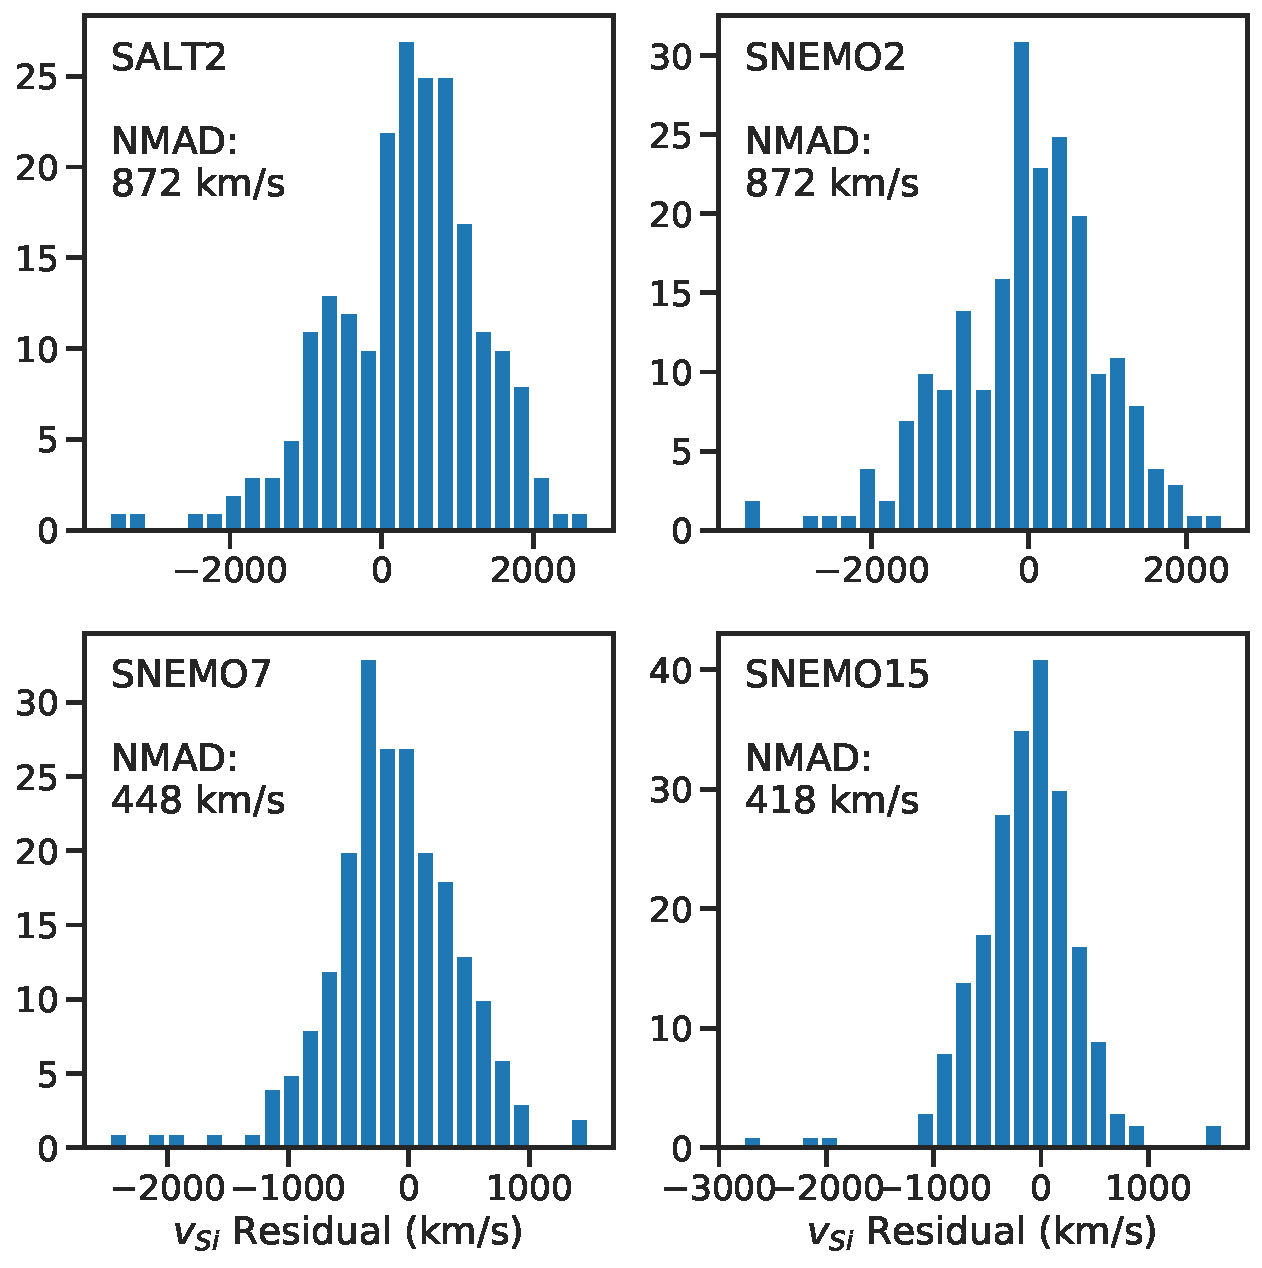
\includegraphics[width=0.9\textwidth]{figures/snemo_kde/model_vSi_recovery.pdf}
    \caption{Histograms of the residuals between the velocity of the SiII6355 line as measured from the data and as measured from the spectrum generated with the best-fit spectral model parameters. Lower dimensional models (SALT2 and SNEMO2) }
    \label{fig:model_vSi_recovery}
\end{figure}

This general trend is seen across all the spectral indicators studied, with the exception of the width of the SiII5972 line; we can see this in Fig. \ref{fig:model_spec_feat_recovery}, where we compare the normalized median absolute deviation ($\text{NMAD}(\bm{x})=1.4826\;\text{med}(|\bm{x}-\text{med}(\bm{x})|)$ of the residuals between model and data spectra for each spectral indicator across spectral models. It is not immediately obvious why the width of the SiII5972 line is captured nearly as well by SALT2 and SNEMO2 as it is by SNEMO15, but not captured by SNEMO7. It may be due to the fact that it is a relatively small feature, and therefore both more difficult to measure precisely on the data spectrum and poorly sampled in the SNEMO spectral eigenvectors. Regardless, we can still claim that SNEMO15 captures all of the spectral indicators studied the best.

\begin{figure}
    \centering
    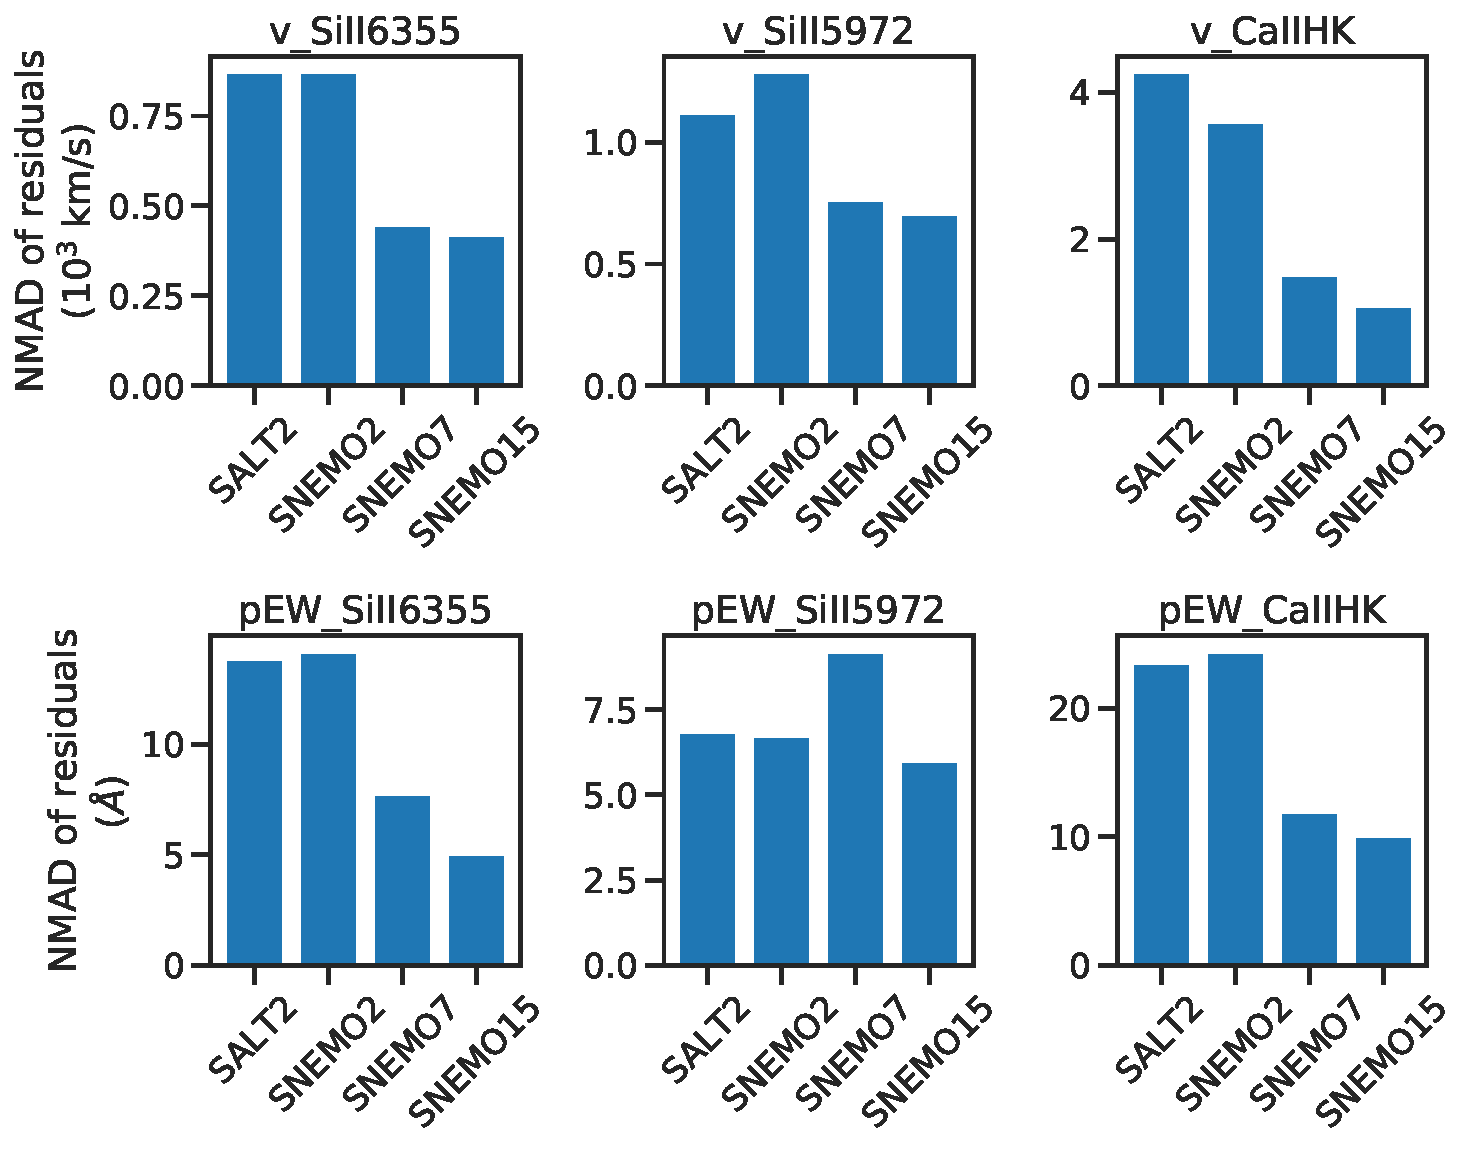
\includegraphics[width=0.9\textwidth]{figures/snemo_kde/model_spec_feat_recovery.pdf}
    \caption{Normalized median absolute deviation of residuals between spectral features measured from data spectra and from spectra generated from the best-fit spectral model. In general, spectral models with more parameters more closely capture the spectral feature measurements.}
    \label{fig:model_spec_feat_recovery}
\end{figure}

\subsection{Comparing Spectral Feature Distributions}
We can also compare the distributions of the spectral indicators seen in generated spectra that do not appear in our data set. To do so, we generate 1000 noiseless, at-max spectra from the KDE model of the spectral feature parameters and the multivariate Gaussian model as explained in Section \ref{sec:making_mocks}, and measure the six spectral indicators for each of these spectra.

The empirical cumulative distributions of the data and the KDE distributions for each of the spectral models are shown in Fig. \ref{fig:ecdf_kde}. A similar plot, but using the multivariate Gaussian model of the spectral model parameter space, is found in Fig. \ref{fig:ecdf_gauss}. These figures look quite similar, though we can pick out some differences (like the difference in the lower velocity portion of SNEMO15 distribution of $v_{SiII5972}$, or the differing relative fractions in each mode of the bimodal $v_{CaIIH\&K}$ distributions for SNEMO15).

\begin{figure}
    \centering
    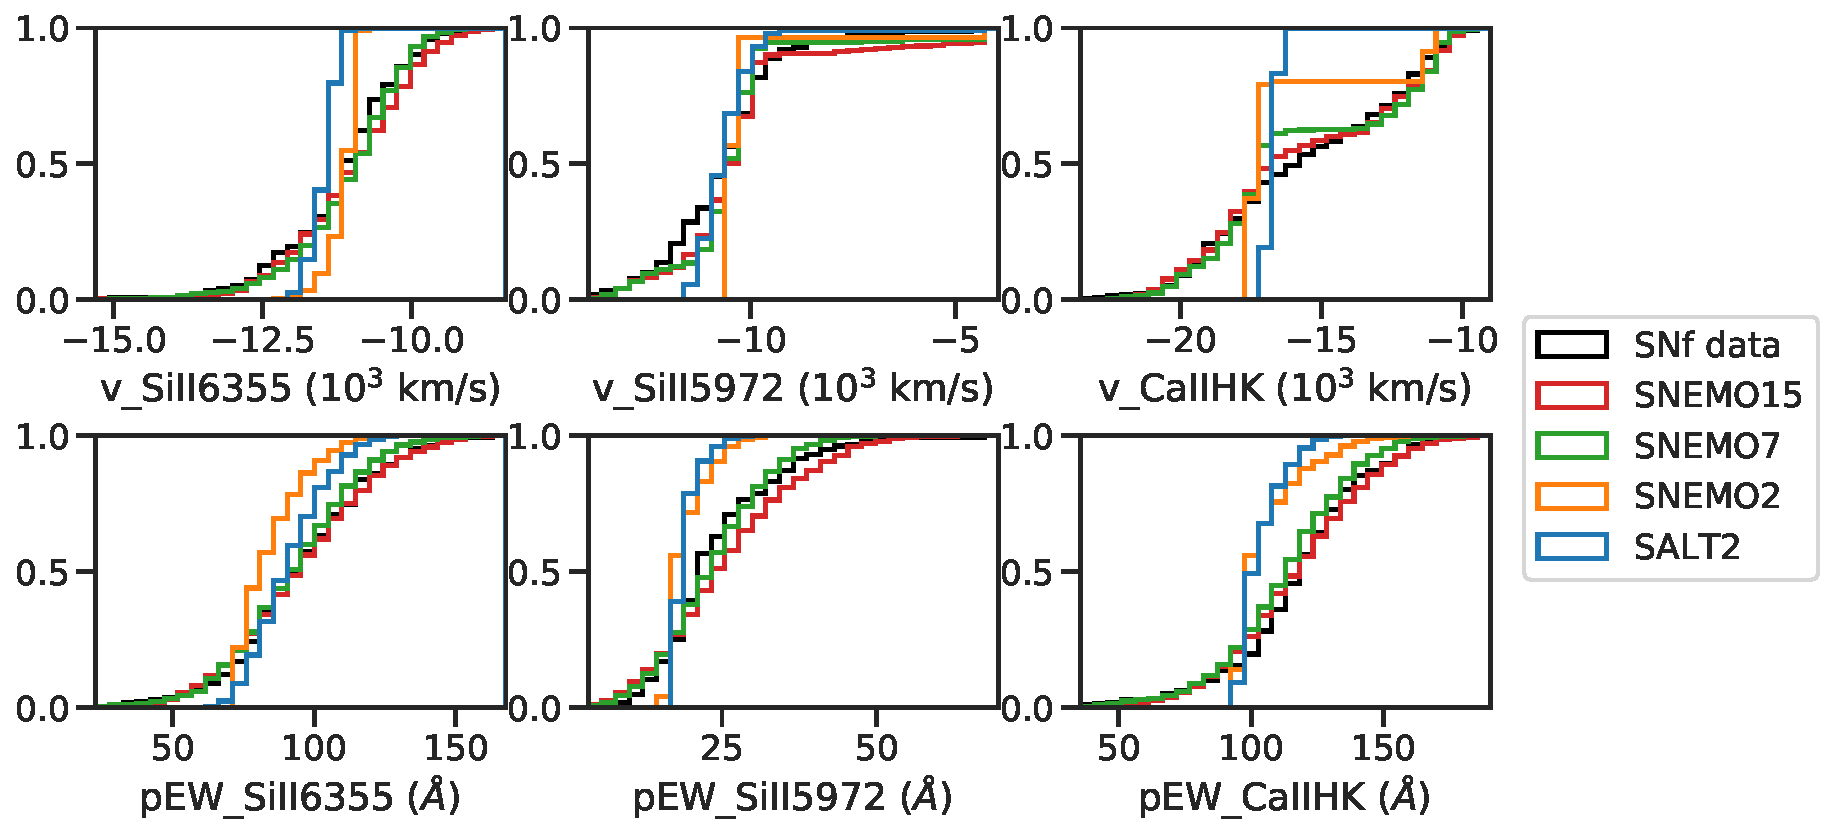
\includegraphics[width=0.9\textwidth]{figures/snemo_kde/ecdf_kde.pdf}
    \caption{Empirical cumulative distribution functions of each spectral indicator for the data set and samples from the kernel density estimate of the spectral model parameter spaces.}
    \label{fig:ecdf_kde}
\end{figure}

\begin{figure}
    \centering
    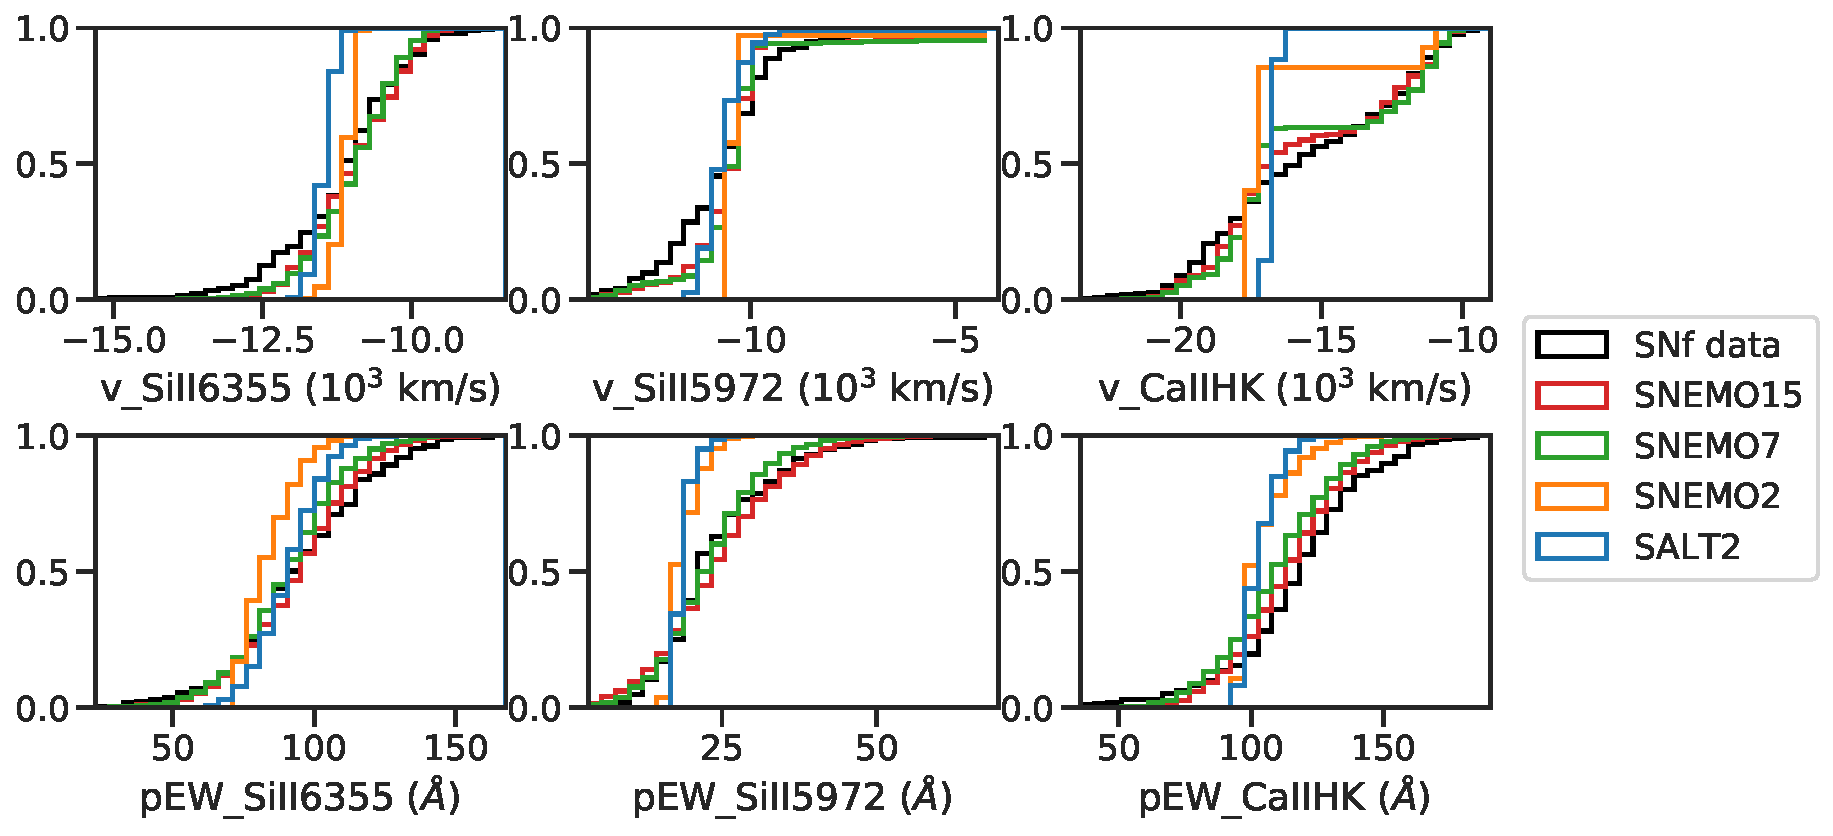
\includegraphics[width=0.9\textwidth]{figures/snemo_kde/ecdf_gauss.pdf}
    \caption{Same as Fig. \ref{fig:ecdf_kde}, but for samples from the multivariate Gaussian estimation of each of the spectral model parameter spaces.}
    \label{fig:ecdf_gauss}
\end{figure}

We can quantify these differences by calculating the Cram\'{e}r distances between the distribution of the data and the distribution of the samples for each feature. We get an estimate of the error on these distances with bootstrap resampling. The resulting distances for the KDE and Gaussian estimates are shown, along with the similarly calculated model to data distances, in Fig. \ref{fig:cramer_spec_feat}. We see a pattern similar to Fig. \ref{fig:model_spec_feat_recovery} in the spectral feature distribution similarity across models -- in every case, spectral models with more parameters have distributions of the spectral indicators that more closely resemble the data. Additionally, for each of the spectral models, the kernel density estimate of the model parameter distributions creates spectral feature distributions that are as or more similar to the true data distribution than the Gaussian estimates and the best-fit parameter spectra. Overall, using more flexible spectral models along with more flexible parameter space models allows for a generative model that can accurately reproduce the full range of spectral behavior for simulations.

\begin{figure}
    \centering
    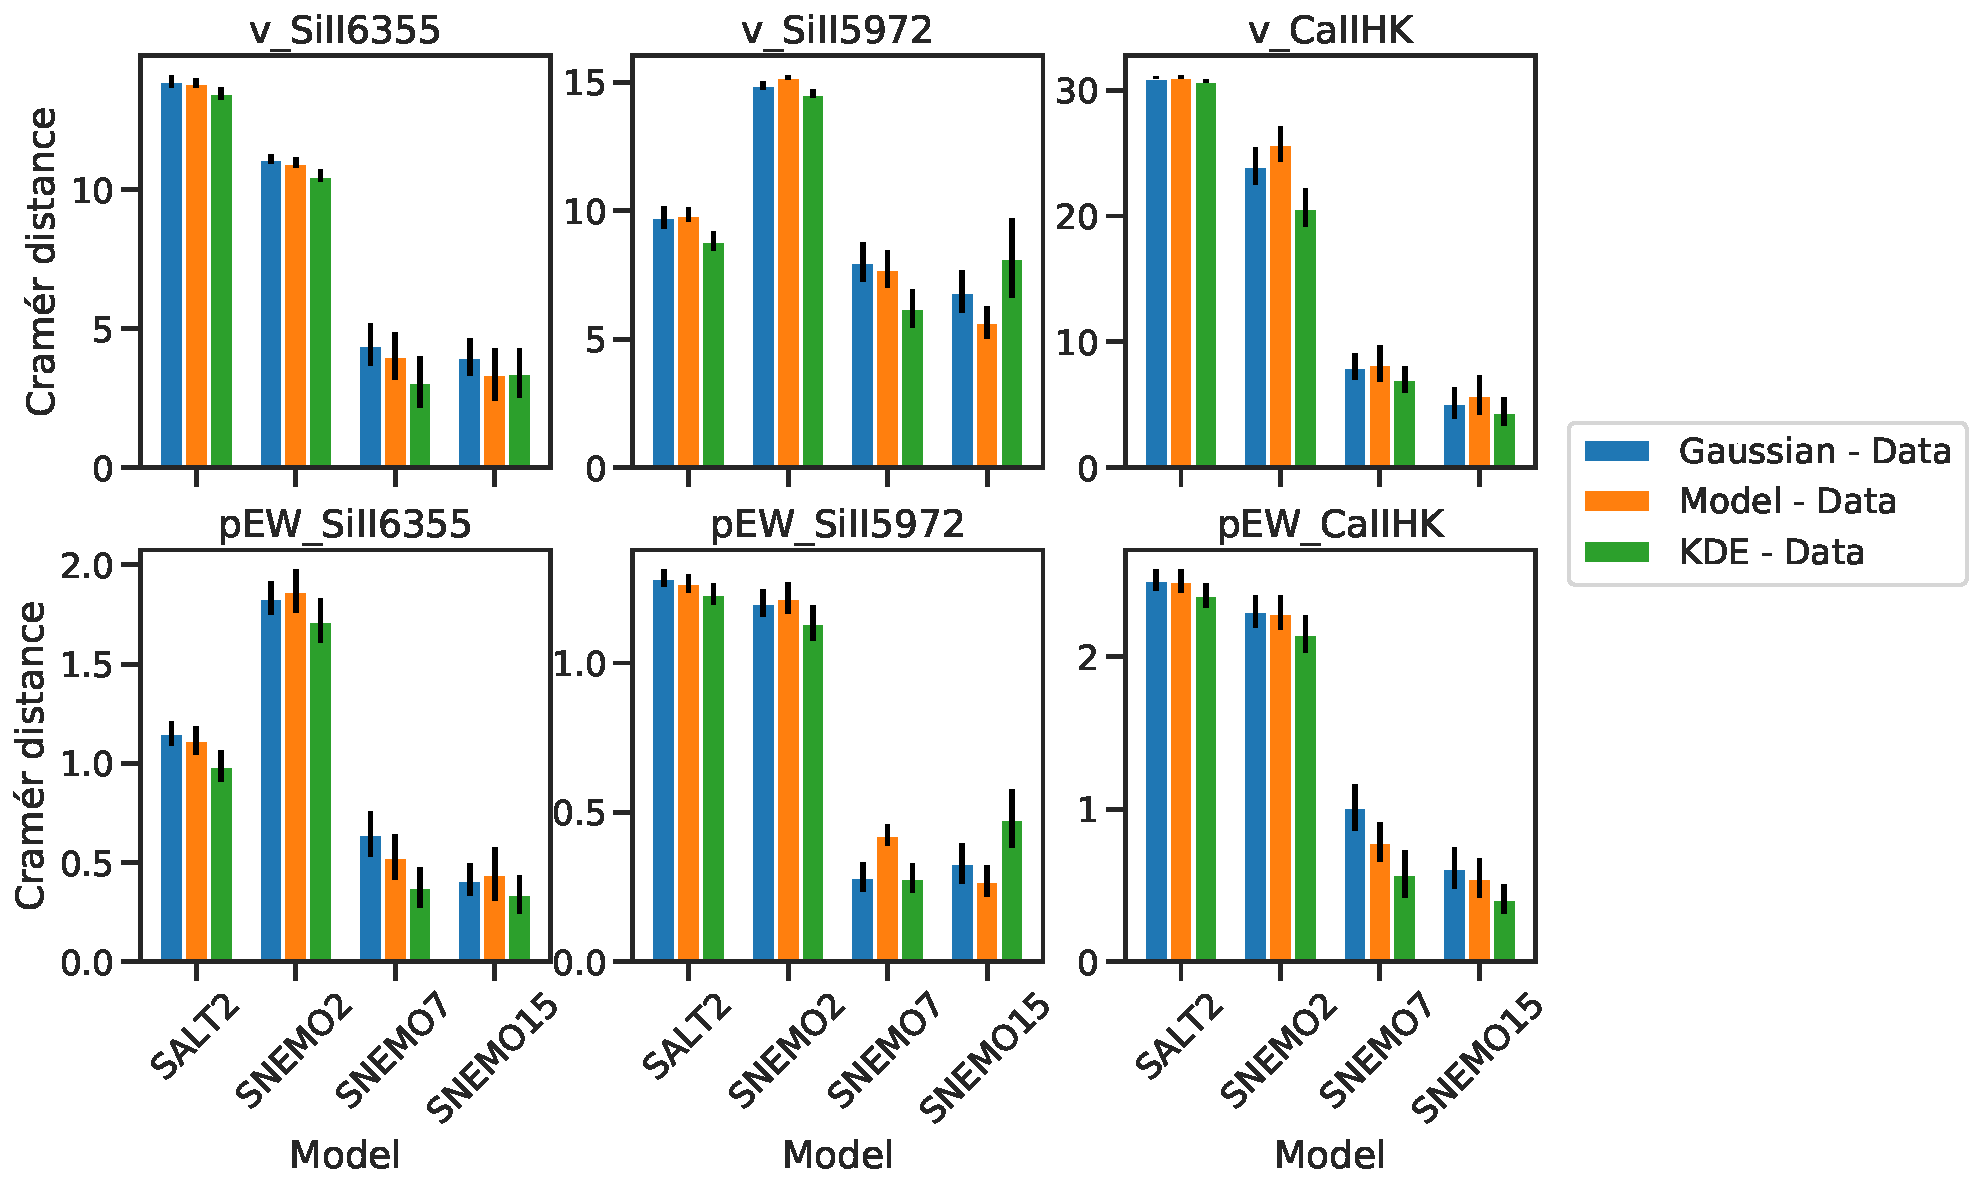
\includegraphics[width=0.9\textwidth]{figures/snemo_kde/cramer_distances_spec_feats.pdf}
    \caption{Cram\'{e}r distances between spectral indicator distributions for the SNfactory data and samples from the KDE estimates of the SALT2 and SNEMO parameter distributions, Gaussian estimates of the spectral model parameter distributions, and the modeled at-max spectra for the training data.}
    \label{fig:cramer_spec_feat}
\end{figure}

\section{Conclusions}
\label{sec:conclusions}
We have presented flexible estimates of the joint probability distributions of model parameters for the SALT2 and the SNEMO models of \cite{Saunders2018}. These estimates can be used to generate synthetic spectra and photometry in simulations that exhibit more spectral diversity than current state-of-the-art simulation techniques. This increased variety makes possible a number of different analyses, from examining the robustness of the twinning technique presented in \cite{Fakhouri2015}, to evaluating spectral feature measurement techniques under different observing conditions. There are a number of spectral properties of Type Ia supernovae beyond the two-parameter light curve shape and color parameters that have been shown to ultimately effect our cosmological parameter measurements. This work presents a simulation tool that properly incorporates these variations, allowing us to properly understand their impacts for future cosmological surveys.

\section{Appendix: Finding a Whitening Matrix}
\label{app:whitening_matrix_proof}
A matrix $W$ that satisfies $W^\top W=\Sigma_X^{-1}$ is a whitening matrix, i.e. if $X$ is a data matrix with covariance $\Sigma_X$, then $Y=WX$ has covariance $\Sigma_Y=\mathbb{I}$.
\begin{align*}
    \textrm{cov}(Y) & = \textrm{cov}(WX)\\
    & = W\textrm{cov}(X)W^\top \\
    & = W\Sigma_X W^\top \\
    & = W(W^\top W)^{-1}W^\top \\
    & = WW^{-1}(W^\top)^{-1}W^\top = \mathbb{I}
\end{align*}

Because the covariance matrix is positive-definite and symmetric, we can diagonalize it, finding a decomposition
$$\Sigma_X = U\Lambda U^T$$
where $\Lambda$ is a diagonal matrix whose entries are the eigenvalues of the matrix and $U^\top U = UU^\top = \mathbb{I}$, where the columns of $U$ are the eigenvectors. Then,
$$\Sigma_X^{-1}=(U\Lambda U^\top)^{-1} = U\Lambda^{-1}U^\top = (\Lambda^{-1/2}U^\top)^\top(\Lambda^{-1/2}U^\top)$$
and thus $W = \Lambda^{-1/2}U^\top$ is a whitening transformation.
